\RequirePackage[dvipsnames,svgnames]{xcolor} % Change font colors
\documentclass[%
  ngerman,        % (ngerman/english) internationalisation
%  listoffigures,  % optional listings of figures, tables and listings
%  listoftables,
%  listoflistings,
%  twoside,        % double sided layout
]{iib_thesis}

\newcommand{\missingQuote}{\textcolor{red}{\underline{\textbf{\uppercase{zitat fehlt}}}}}

% Add `diff` language for lstlisting
  \definecolor{diffstart}{named}{Grey}
  \definecolor{diffincl}{named}{Green}
  \definecolor{diffrem}{named}{OrangeRed}

  \lstdefinelanguage{diff}{
    basicstyle=\ttfamily\small,
    morecomment=[f][\color{diffstart}]{@@},
    morecomment=[f][\color{diffincl}]{+\ },
    morecomment=[f][\color{diffrem}]{-\ },
    numbers=left,
  }

\title{Entwicklung eines erweiterbaren Kommandozeileninterfaces zur Generierung von Web-Applikationen}
\author{Michael David Kuckuk}
\degree{Bachelor}
\studyprogram{Angewandte Informatik}
\date{\today}
\matno{108 017 207 503}
\firstadviser{Prof. Dr.-Ing. Markus König}
\secondadviser{Stephan Embers, M.\,Sc.}
\myabstract{
The ABSTRACT is to be a fully-justified text following the title page. The text will be formatted in 12\,pt, single-spaced Computer Modern. The title is ``Abstract'', set in 12\,pt Computer Modern Sans Serif, centered, boldface type, and initially capitalized. Writing the abstract in English is mandatory even if the thesis itself is written in German. The length of the abstract should be roughly about 200 words but must not exceed 250 words.

As usual, the abstract should clearly summarize the aim, the background and the results of your thesis so that an interested reading can decide if he or she wants to further read your (interesting) written report. Also, the abstract should be kept simple. That is, do not include tables, figures or cross references in the abstract. You will have plenty of time in your thesis to explain things more clearly.
}

\begin{document}

  \newacronym{CLI}{CLI}{Command Line Interface}
\newacronym{CRA}{CRA}{create-react-app}
\newacronym{TS}{TS}{TypeScript}
\newacronym{JS}{JS}{JavaScript}
\newacronym{npm}{NPM}{Node Package Manager}
\newacronym{MVC}{MVC}{Model View Controller}
\newacronym{DOM}{DOM}{Document Object Model}
\newacronym{VCS}{VCS}{Versionskontrollsystem bzw. Engl.: Version Control System}
\newacronym{JSON}{JSON}{JavaScript Object Notation}

  \section{Einleitung}
Entwickelnde haben zu Beginn eines neuen Projektes immer erst die Aufgabe, sich eine geeignete Architektur für das Projekt zu überlegen, die sie dann möglichst von Anfang an verfolgen können. In den meisten Programmiersprachen und Umfelden -- insbesondere in der Webentwicklung -- ist ein Teil dieser Aufgabe die Auswahl von Bibliotheken und Werkzeugen, die bei der Programmierung von Nutzen sein könnten.

Unter diesen Bibliotheken und Werkzeugen gibt es viele, die besonders häufig verwendet oder in bestimmten Kombinationen empfohlen werden. Beispielsweise verwenden 60,4\% der von \glqq State of JS 2020\grqq\ Befragten die Bibliothek Axios\footnote{\url{https://www.npmjs.com/package/axios}} (ein HTTP-Client, der für Browser und Node.js dasselbe Interface bietet). Unter den Befragten nutzen 89,6\% das Werkzeug \gls{npm}\footnote{\gls{npm} genießt jedoch als offizieller Node.js-Paketmanager eine Sonderstellung. Daher ist diese Zahl nur begrenzt mit anderen Verwendungsquoten vergleichbar.}, 82,3\% nutzen ESLint\footnote{\url{https://www.npmjs.com/package/eslint}} (ein Werkzeug zur statischen Codeanalyse) und 70,9\% nutzen Prettier\footnote{\url{https://www.npmjs.com/package/prettier}} (ein Codeformatierer) \cite{stateofjs}.

Die genauen Konstellationen, in der diese Bibliotheken und Werkzeuge verwendet werden, unterscheiden sich jedoch von Projekt zu Projekt. Sie hängen primär von den Anforderungen des Projekts ab, aber variieren auch je nach persönlicher Präferenz oder aufgrund von Empfehlungen, die in offiziellen Dokumentationen ausgesprochen werden. Beispielsweise wird empfohlen, Angular zusammen mit TypeScript zu verwenden \cite{angular_only_with_typescript}.

Nachdem entschieden wurde, welche Konstellation von Bibliotheken und Werkzeugen zu verwenden ist, müssen diese im nächsten Schritt installiert werden und miteinander verknüpft werden, sodass sie alle zusammen funktionieren. Dieser Schritt unterscheidet sich von klassischen Entwicklungsaufgaben, da hierbei Probleme wie Laufzeitanalyse oder Graphentheorie keine Rolle spielen. Stattdessen müssen Konfigurationsdateien erzeugt, Objekte in gewissen Reihenfolgen initialisiert und Werkzeuge in den Kompilierprozess eingebunden werden, der je nach Konstellation der Werkzeuge zunächst eingerichtet werden muss.

Ziel dieser Arbeit ist es, diese initiale Projektgenerierung zu automatisieren. Über ein \gls{CLI} sollen zunächst einige Fragen gestellt werden, durch die festgestellt wird, welche genaue Konstellation von Bibliotheken und Werkzeugen installiert werden soll. Entsprechend dieser Spezifikation soll dann ein Projekt erzeugt werden, in dem keine weitere Verdrahtung mehr notwendig ist und in dem sofort alle Bibliotheken und Werkzeuge verwendet werden können.

Es gibt bereits mehrere Projekte, die sich ebenfalls dieser Aufgabe widmen und auf die im späteren Verlauf der Arbeit näher eingegangen wird. Diese haben jedoch den Nachteil, dass sie nur begrenzte Unterstützung für Bibliotheken und Werkzeuge liefern. Manche der Projekte bieten eine Möglichkeit zur Erweiterung um neue Bibliotheken und Werkzeuge an, jedoch sind derartige Erweiterungen nicht schon bei der Projektinitialisierung verwendbar und müssen daher in weiteren Schritten nach der Initialisierung ausgeführt werden.

Neben der beschriebenen Erleichterung des Installationsprozesses bieten derartige \gls{CLI}s auch den Vorteil, dass sie Einsteigenden bei der Entdeckung neuer Werkzeuge und Bibliotheken helfen können. Im Jahr 2019 gab es bereits über 1,3 Millionen \gls{npm}-Pakete \cite{npm_package_count}. Diese Zahl erschwert besonders am Anfang das Auswählen sinnvoller Pakete.

Durch ein \gls{CLI} kann eine Vorauswahl dieser Pakete getroffen werden, die leichter von Einsteigenden überblickt werden kann. Zudem können der Vorauswahl weitere Informationen wie Abhängigkeiten zwischen Bibliotheken oder Links zu zugehörigen Dokumentationsseiten angehängt werden, die das Treffen einer Auswahl zusätzlich erleichtern.

Im Rahmen dieser Arbeit wird daher ein solches \gls{CLI} namens \gls{GWA} entwickelt. Es soll in der Lage sein, leicht verständliche Fragen zu stellen und basierend auf den Antworten ein funktionsfähiges Projekt zu erzeugen. Bei der Konzeptionierung und Entwicklung wird ferner darauf geachtet, dass \gls{GWA} leicht erweitert werden kann, um die Einbeziehung zukünftiger oder zum Entwicklungszeitpunkt nicht berücksichtigter Bibliotheken und Werkzeuge zu ermöglichen.

Bevor mit der Konzeptionierung von \gls{GWA} begonnen wird, wird der jetzige Stand der Technik erläutert. Dies umfasst neben einigen Grundlagen, die zum besseren Verständnis der Arbeit beitragen, eine Vorstellung der bereits erwähnten Projekte mit ähnlicher Zielsetzung.

Daraufhin wird analysiert, welche Anforderungen genau von \gls{GWA} erfüllt werden sollen. Hierfür werden zunächst die Vor- und Nachteile der bereits existierenden Projektgeneratoren analysiert. Daraufhin wird eine Auswahl der zu verwendenden Technologien getroffen und es werden erste Pläne zur Gestaltung des Ablaufs und des Datenmodells angefertigt.

Der Fokus der Arbeit liegt auf der Implementierung von \gls{GWA}. In diesem Zusammenhang wird das allgemeine Vorgehen bei der Entwicklung erläutert. Es werden einige zentrale Probleme untersucht, für die verschiedene Lösungsoptionen ausgearbeitet und diskutiert werden und von denen anschließend eine ausgewählt und umgesetzt wird.

Abschließend wird evaluiert, ob die gesetzten Ziele erfüllt werden konnten. Es wird diskutiert, welche Probleme weiterhin bestehen und womit sich zukünftige Forschung auseinandersetzen könnte.
%  % !TEX root = ../thesis.tex

\section{Layout}

The layout of the title page is as shown on the title page of this document. It contains the thesis' title bordered by horizontal edges, information about the student, and information about the supervisors.

All pages except the title page and the abstract are numbered. Numbers are placed on the pages' outer sides. Indicies are numbered in roman numerals whereas the rest is numbered in arabic numerals.

Sections are numbered automatically. You can write sections and subsections to structure your text (using the corresponding LaTeX keywords). If necessary, you can further use a ``subsubsection'' keyword, but that should be enough.

  \subsection{Structure}
  The structure of a thesis is as follows:

  \begin{itemize}
      \item Title page
      \item Declaration
      \item Abstract
      \item Table of Contents
      \item Thesis Specific Structure of Sections
      \item Lists of Figures, Tables, Listings (only if absolutely necessary)
      \item References
		\item Appendex (only if necessary)
  \end{itemize}

\section{Formatting}

	All text is in single-column format. It is fully-justified 12\,pt Computer
Modern. The Table of Contents--depth is set to 2, so even if there are deeper
subsections, they not included in the Table of Contents.

  \subsection{Figures and Tables}

  Figures can be placed in your text to show some interesting stuff. In the simplest case, use the floating ``figure'' environment with a good caption (see Fig. \ref{fig:example}).

  \begin{figure}
		\centering
		
\includegraphics[width=0.5\textwidth]{cat.jpeg}
      \caption{A picture of a cat, the second most popular Internet theme.}
		\label{fig:example}
  \end{figure}

  Figures should not contain code, use listings (see section \ref{subsec:listings}) instead. Captions contain a full description of the figure including parameters and color codes if not given within the figure. All figures have to be referenced in the text. Subfigures are alphabetically enumerated where the letters are parenthesized.  Caption are written \textit{below} figures, but \textit{above} tables (see Table \ref{tab:example}).

  \begin{table}
	  \centering
	  \caption{A simple table example using the \textit{tabularx} package}
	  \begin{tabularx}{0.4\textwidth}{cr}
		  \textbf{Pet Type} & \textbf{Price [EUR]}\\
		  \hline
		  cat & 33.00 \\
		  dog & 22.00 \\
		  guinea pig & 11.00 \\
		  \hline
	  \end{tabularx}
	  \label{tab:example}
  \end{table}

  \subsection{Equations}
  All equations have to be referenced in the text and should be written as LaTeX math code and not included as an image. See any LaTeX math tutorial how to do this, for example the Wikipedia book on this subject: \url{https://en.wikibooks.org/wiki/LaTeX/Mathematics}.

  \subsection{Listings}
  \label{subsec:listings}

	All listings should be referenced in the text. There is a \textit{listings} package that can you can use to clearly show some code snippets in your text. See the CTAN website for more details: \url{https://ctan.org/pkg/listings}. In any case, listings should be used sparsely, use pseudo-code instead of source code where applicable.

  \subsection{References}

	When you refer to another publication or a website in your thesis, you must give a proper reference using Bibtex. You can cite a book, for example the LaTeX book by Leslie Lamport \cite{lamport2005}; or a conference paper, for example one given at Oulu, Finnland \cite{hilfert_koenig_2015}; or a paper in a journal, for example a paper in ``Visualization in Engineering'' \cite{hilfert_koenig_2016}.

	Citing a website (URL) is OK, but include as much information as possible, not just the URL \cite{wiki:xxx}.

	\subsection{Appendix}

	\begin{itemize}
		\item
			Lots of pictures and diagrams...
		\item
			Lots of important pieces of program code...
		\item
			Long tables of important, but boring, numbers...
		\item
			Anything else which is important, but will hinder the reading in
			the main text...
	\end{itemize}

%  % !TEX root = ../thesis.tex

\section{Structure of scientific work}
In order to ensure a systematic structure, scientific work should be structured similarly to the structure described below. In addition to the cover page and the declaration of authorship, scientific papers usually include at least one index of contents, illustrations and tables as well as a list of abbreviations, followed by the actual main part and a bibliography. In general, it should be noted that a reasonable structure depends to a large extent on your topic and your chosen method. Thus, the structure of literature reviews, conceptual work and development work usually differs from each other.

\subsection*{Summary or Abstract}
The summary or abstract is detached from the actual elaboration and contains, in addition to a description of the task or objective, in particular the procedure, the methods applied as well as the essential results and summarises them as briefly as possible. The Summary or Abstract is not part of the structure of the work and therefore is not numbered.

\subsection*{Table of Contents}
The table of contents includes all first, second and third level headings listed later in the work. A deeper structure than in the third level is to be avoided in the context of scientific work. In this context, the bibliography and the appendix are included as first level headings in the structure and thus in the table of contents, but are not numbered. The table of contents is not included in the structure of the work and is explicitely not numbered!

\subsection*{Optional: I List of Figures}
The list of figures lists all the illustrations and figures used in the work, including the caption and the corresponding page numbers (preset in this template). The list of figures is the first list with an independent, otherwise Roman section numbering. This list only needs to be appended when necessary. In individual cases, it may be helpful to consult the work supervisor.

\subsection*{Optional: II List of Tables}
The list of tables lists all the tables used in the work, including their labels and the corresponding page numbers (preset in this template). This list only needs to be appended when necessary. In individual cases, it may be helpful to consult the work supervisor.

\subsection*{Optional: III List of Formulas}
The list of formulas lists all formulas used in the work, including the label and the corresponding page number. It is only necessary if there are at least 3 or more formulas used in the work. This list only needs to be appended when necessary. In individual cases, it may be helpful to consult the work supervisor.

\subsection*{Optional: IV List of Abbreviations}
The list of abbreviation lists all abbreviations used in the work, including their definition. This list only needs to be appended when necessary. In individual cases, it may be helpful to consult the work supervisor.

\subsection*{Optional: V List of Symbols}
The list of symbols lists all mathematical symbols used in the work, including their definition. This list only needs to be appended when necessary. In individual cases, it may be helpful to consult the work supervisor.

\subsection*{1 Introduction}
Within the introduction, the objective is formulated, placed in an superordinate context and distinguished from other topics. The most important terms of the topic must be placed within the context to be considered in the introduction while an thorough formulation is particularly important. In addition, information on the methodology can be provided. The structure of the work should be presented. 

Thus the first section contains the following aspects:

\begin{itemize}
	\item Description of the problem to be solved with this work
	\item Objective of the work and the delivered contribution to science
	\item Structure of the work
\end{itemize}

In the case of extensive scientific work, such as bachelor's and master's theses, the introduction should consist of one to three pages. In addition, it is useful to insert a figure at the end of the section which shows the structure, the argumentative sequence or important core statements of the work. Experience shows that the introduction should only be formulated in detail at the end of the work in order to avoid repeated changes to the main text.

\subsection*{2 Related Work}
Based on the introductory explanations, this section focuses on the contextualisation of the problem or objective described and the synthesis of the necessary fundamental principles. Necessary fundamental principles contain knowledge on topics that cannot be assumed to be engineering knowledge in the field of construction sciences or computer science.

In this context it is important to explain elementary terms, definitions and/or theories on the one hand and to present the state of research in the respective subject area on the other hand.
Accordingly, a summary is given of the scientific basis on which the scientific work to be written is based.

\subsection*{3 Methodology}
This section focuses on the methodology chosen to achieve the research objectives or to answer the research questions. It is made clear how the objective of the work formulated in the introduction is to be achieved or implemented using scientific methods.

\subsection*{4 Additional Main Section(s)}
In general, this main section or sections represents your results. The concrete structure of the scientific work depends largely on the task to be solved or the research questions to be answered, so that no detailed recommendations for this section can be given here, but exemplary sections could be requirements analysis, conception, development, evaluation for a development work or test setup, test execution, evaluation for an experimental work. For the specific structuring of the main section(s) a consultation with the supervisor of the work is helpful in any case.

\subsection*{5 Discussion}
The discussion serves to interpret or critically discuss the results achieved on the basis of the problem or question formulated in the introduction as well as in the context of current and relevant literature on the topic. In this context, unexpected results or contradictions to assumptions made or to the existing scientific literature will be specifically worked out.

\subsection*{6 Conclusion}
The conclusion completes the scientific work as a final statement. The objective, the methodology applied and the conclusions drawn are summarised once again and assessed in terms of the extent to which the introductory objective could be achieved. It is advisable to consider possible limitations of your work and to reflect critically on your approach. In addition, you should formulate in an outlook how further scientific work could tie in with its results and which priorities you see for further research work in the topic area of your work.

\subsection*{Bibliography}
In the bibliography, all sources used in the context of scientific work are specified in detail.

\subsection*{Appendix}
In principle, only those contents are included in the appendix which are not essential for the understanding of the content, but which may have an important relation to the own elaborations or an additional information character. These include, for example, questionnaires specially developed for the purpose of a study.


  \section{Stand der Technik}
Um die Implementierung der Arbeit vollständig nachvollziehen zu können, ist es wichtig, einige Konzepte verstanden zu haben und zu wissen, worauf die Entwicklung aufbauen wird. Diese Grundlagen werden im Folgenden eingeführt und erläutert.

\subsection{Kommandozeileninterfaces}
Die erste weitverbreitete Art von Computerprogrammen waren sogenannte Kommandozeileninterfaces (\gls{CLI}s). In der Kommandozeile konnten diese Programme über ihren Namen bzw. ihren Speicherort aufgerufen werden, wobei zusätzliche Argumente übergeben werden konnten, um den Ablauf des Programms zu beeinflussen \cite{verma2013gracoli}.

Diese Nutzweise birgt verschiedene Vor- und Nachteile. A priori bietet sie keine Entdeckbarkeit für verschiedene Funktionalitäten eines Programms. Erst durch die Einrichtung eines weiteren Befehls bzw. einer Konfigurationsoptionen kann Nutzenden anstelle der ordinären Ausführung des Programms eine Liste aller seiner Nutzungsmöglichkeiten angezeigt werden. Nutzende müssen aber auch diesen Befehl kennen, um ihn ausführen zu können.

Dafür lassen sich derartige Befehle sehr leicht automatisiert ausführen, da sie ohne Weiteres in Skripte eingebunden werden können. Um eine automatische Ausführung grafischer Benutzeroberflächen zu ermöglichen, müsste hingegen die Benutzung einer Computermaus oder Tastatur simuliert werden \cite{fellmann2007command}.

Seit diesen Anfängen von \gls{CLI}s ist es jedoch möglich geworden, im Rahmen eines \gls{CLI}s weitere Nutzereingaben wie die Verwendung von Tastatur und Maus zu verarbeiten. So können Nutzerinteraktionen ermöglicht werden, die einer grafischen Benutzeroberfläche gleich kommen. Beispielsweise ist es möglich, sich in der Kommandozeile eine Weltkarte anzeigen zu lassen, die mit Maus und Tastatur bedienbar ist \cite{mapscii}.

Heutzutage bieten \gls{CLI}s daher den Vorteil, dass sie weiterhin leicht automatisierbar sind und dennoch Interaktivität und damit Entdeckbarkeit der Funktionen ermöglichen. Um die Umsetzung derartiger Interaktivität zu erleichtern, gibt es zahlreiche Bibliotheken.

\subsection{Einführung in Frontend-Frameworks für Webapplikationen}
Die Entwicklung interaktiver Webapplikationen erfolgt mittels HTML, CSS und JavaScript. Browser stellen den mit HTML definierten Inhalt dar, manipulieren das Aussehen der Seite anhand der durch CSS definierten Regeln und verfügen zudem über einen JavaScript Interpreter, der den übermittelten JavaScript Code ausführen kann und dadurch~ eine Manipulation der Seiteninhalte erlaubt.

Durch diese Möglichkeit ergibt sich das Problem, dass die Daten, die das Programm berechnet (oder auf andere Weise erlangt) Nutzenden korrekt dargestellt und umgekehrt Eingaben von Nutzenden in den Daten widergespiegelt werden sollen.

Beim Entwickeln solcher Funktionalität wiederholen sich häufig bestimmte Probleme wie die Synchronisierung von Daten mit der Anzeige oder die Wiederverwendung von Teilen der Nutzeroberfläche. Diese Probleme können mithilfe von Frontend-Frameworks gelöst werden.

Zur Zeit gibt es vor allem drei Frameworks, die häufig verwendet werden: React, Angular und Vue \cite{stateofjs}. Angular und Vue bauen dabei auf dem \gls{MVVM}-Pattern auf \cite{angular_mvvm}. Dort kann jeweils in einer Variation von HTML, in der bestimmte JavaScript- bzw. TypeScript-Ausdrücke interpretiert werden können, die View aufgebaut werden. Die Funktionalität des ViewModels wird in einem zur View gehörenden JavaScript- bzw. TypeScript-Block implementiert und das Model kann über weitere Klassen dargestellt werden. Während in Angular View, ViewModel und Model in verschiedene Dateien aufgeteilt werden, sind in Vue die View und das ViewModel in derselben Datei zu vereinen.

React hingegen verfolgt nicht so strikt das \gls{MVVM}-Pattern. Hier wird durch die freiwillige, aber empfohlene Verwendung zusätzlicher Syntax ermöglicht, eine Variante von HTML-Ausdrücken in JavaScript bzw. TypeScript einzufügen, die dann wie andere Werte auch in Variablen gespeichert werden können \cite{react_jsx}. Auf diesem Weg wird parallel zum eigentlichen \gls{DOM} ein sogenanntes Virtual \gls{DOM} generiert, das dann in das eigentliche \gls{DOM} überführt wird. Somit ist es in React möglich, View und Controller komplett miteinander zu vereinen.

Alle drei dieser Frameworks ermöglichen eine komponentenbasierte Entwicklung. Das bedeutet, dass mit sehr geringem Aufwand die View in Komponenten unterteilt werden kann, die dann wiederverwendet werden können.

Aus diesen und weiteren Gründen verwenden die meisten Webentwickelnden Frontend-Frameworks, um darauf ihre Projekte aufzubauen \cite{stateofjs}. Da jedes Framework aber mehr oder weniger klare Strukturen, Datenflüsse, Syntaxen und vieles mehr vorgibt, ist die Entscheidung eines Frameworks in Bezug auf die Suche weiterer Abhängigkeiten eine sehr folgenschwere Entscheidung.

Beispielsweise ist es im Rahmen der empfohlenen Installationsprozesse nicht möglich, Angular ohne TypeScript oder React ohne ESLint zu verwenden \cite{angular_only_with_typescript} \cite{react_eslint}. Für alle drei der genannten Frameworks gibt es Komponentenbibliotheken\footnote{Material-UI für React: \url{https://material-ui.com/}; Angular Material für Angular: \url{https://material.angular.io/}; Vuetify für Vue: \url{https://vuetifyjs.com/en/}}, die Google's Material Design System folgen; allerdings sind diese Bibliotheken sehr verschieden, haben unterschiedliche Features und gehen nicht aus demselben Code hervor.

Die Entscheidung eines Frameworks ist daher eine der ersten Entscheidungen, die Entwickelnde beim Einrichten ihrer Projekte treffen müssen. Sie schränkt die weitere Auswahl an Werkzeugen und Bibliotheken ein. Außerdem können, bis auf in besonderen Kontexten wie Micro-Frontends oder WebComponents, nur mit hohem Aufwand oder gar nicht zwei Frameworks zusammen verwendet werden.

\subsection{Ähnliche Projektgeneratoren}
Um das Problem der initialen Projektkonfiguration zu automatisieren oder zumindest zu erleichtern, bieten die drei oben erwähnten Frameworks jeweils ein Programm an, was zur initialen Erstellung von Projekten mit dem jeweiligen Framework empfohlen wird. Einige dieser Programme sind darüber hinaus in der Lage, auch nach dieser initialen Erstellung Änderungen am Code vorzunehmen. Diese Funktionalität ist jedoch für \gls{GWA} nicht geplant und wird daher nicht näher betrachtet.

\subsubsection{React}
In der Dokumentation für React wird empfohlen, neue Projekte über das \gls{CLI} \gls{CRA} zu erstellen. Dieses kann per \gls{npm} installiert werden und ist dann in der Lage, den Inhalt eines angegebenen Templates (oder eines Standardtemplates) in ein spezifiziertes Verzeichnis zu kopieren. Daraufhin werden die benötigten Abhängigkeiten per \gls{npm} oder mittels eines anderen installierten Paketmanagers (wie z.B. Yarn\footnote{\url{https://yarnpkg.com/}}) installiert.

Dritten ist es möglich, eigene Templates für \gls{CRA} zu erzeugen, die dann wie Erstanbietertemplates zur Erzeugung des neuen Projekts genutzt werden können. Wenn also mittels \gls{CRA} ein Projekt erzeugt werden soll, das bereits bei seiner Erzeugung mit gewissen Bibliotheken oder Werkzeugen ausgestattet wird, muss dafür zuvor ein entsprechendes Template erstellt worden sein. Die Wahrscheinlichkeit, dass dies jedoch bereits geschehen ist, sinkt mit der Spezifität der Wünsche.

Die Erstanbietertemplates geben bereits die empfohlene Ordner- und Dateistruktur für React-Projekte vor; durch Drittanbietertemplates kann hiervon aber abgewichen werden. Außerdem installieren die Erstanbietertemplates bereits einige weitere Werkzeuge wie ESLint, Jest (ein Werkzeug zum Schreiben und Ausführen von automatisierten Tests; siehe Kapitel \ref{konz:jest_explanation}) und die sogenannten react-scripts. Diese sind eine Sammlung von kleinen Skripten und Abhängigkeiten, die Prozesse automatisieren, die für die Entwicklung notwendig sind. Beispielsweise wird hierüber ein Skript zur Verfügung gestellt, welches einen lokalen Server startet, der den aktuellen Stand der Webapplikation hostet und bei jeder Codeänderung automatisch aktualisiert. Dieser Server gibt zudem auch die Warnungen aus, die ESLint erzeugt.

Außerdem ist es bei der Verwendung dieser Templates mit geringem Aufwand möglich, bestimmte empfohlene Bibliotheken und Werkzeuge nachzurüsten. So gibt es zum Beispiel Anleitungen für die Installation von Prettier oder von CSS-Präprozessoren, die aus jeweils einem in der Kommandozeile auszuführenden Befehl bestehen. Für Prettier muss zudem noch eine bestimmte, bereits existierende Datei um einige vorgegebene Zeilen ergänzt werden.

\subsubsection{Angular}
Das Angular-Team stellt das sog. Angular-\gls{CLI} zur Verfügung, das Entwickelnden beim Programmieren verschiedene wiederkehrende und repetitive Aufgaben abnehmen soll (wie z.B. die Erstellung und Einbindung neuer Komponenten). Neben diesen Aufgaben wird das Tool auch zur Erzeugung neuer Angular-Projekte genutzt.

Der Befehl \verb|ng new <project-name>| führt Nutzende in einen Dialog, bei dem zwei Fragen zur gewünschten Konfiguration des Projektes gestellt werden. Über explizit gesetzte Kommandozeilenoptionen können weitere Features konfiguriert werden, mit denen das Projekt eingerichtet wird. Diese Features sind jedoch allesamt Angular-intern, d.h. es gibt keine Möglichkeit weitere Bibliotheken oder Ähnliches installieren zu lassen, die nicht direkt vom Angular Team kommen. Selbst einige Bibliotheken (z.B. Angular Material), die vom Angular-Team direkt entwickelt werden, sind nicht in diese initiale Projektgenerierung eingebunden. Eine Ausnahme hiervon bildet die Auswählbarkeit der CSS-Präprozessoren SCSS, Sass und Less.

Im Gegensatz zu \gls{CRA} sind hier die Möglichkeiten, die Nutzenden bei der initialen Projekterstellung geboten werden, sehr eingeschränkt. Es gibt die Möglichkeit, bei der Einrichtung eine sogenannte \glqq Collection\grqq\ anzugeben, die dann die Erstellung des eigentlichen Projektes übernimmt. Es könnte also eine Collection entwickelt werden, die weitere Bibliotheken je nach Eingabe einbindet. Jedoch scheint die Umsetzung dieses Features abzunehmen: von den überprüften Collections für ESLint, Prettier und Apollo-Angular hat nur eine dieses Feature (also die Installation während statt nach der Initialisierung) jemals unterstützt. Mittlerweile ist aber auch diese Unterstützung eingestellt worden \cite{prettier_angular_collection_file} \cite{angular_eslint}\footnote{Dies verdeutlicht insbesondere folgender Kommentar des Projekteigentümers: \url{https://github.com/angular-eslint/angular-eslint/issues/395\#issuecomment-821991202}} \cite{apollo_angular_collection_file}.

Im Gegensatz zu der React-Lösung können sich Nutzende hier (im Rahmen der beschränkten angebotenen Optionen) eine beliebige Konfiguration aussuchen und sind nicht darauf angewiesen, dass jemand vor ihnen schon denselben Wunsch hatte. Außerdem wird durch die gestellten Fragen auch Anfänger:innen die Entdeckung empfohlener Pakete und der Einstieg in Angular erleichtert, da ihnen gewisse Features automatisch vorgestellt werden.


\subsubsection{Vue}
Von den drei Frameworks bietet Vue in Bezug auf die Projekterstellung das umfangreichste \gls{CLI}. Zuallererst besteht die Möglichkeit, ein Preset auszuwählen. Dies kann eines von zwei Standardpresets sein oder eines, das zuvor auf dem lokalen Computer erstellt und gespeichert wurde. Es ist auch möglich, ein bereits existierendes Preset oder ein komplett neues Preset als Kommandozeilenparameter anzugeben, um diese Frage zu überspringen.

Falls kein Preset ausgewählt wird, ist zunächst im Rahmen einer Multiple-Choice-Frage eine Vorauswahl von zehn Features zu treffen, die im Projekt gewünscht bzw. nicht gewünscht sind. Daraufhin werden zu den ausgewählten Features detailliertere Fragen gestellt. Insgesamt stehen durch das Vue-\gls{CLI} Tool über 20 verschiedene Bibliotheken bzw. Werkzeuge ohne weiteren Konfigurationsaufwand zur Verfügung. Die soeben erstellte Konfiguration kann anschließend als neues Preset gespeichert werden.

Wie im Angular-\gls{CLI} können auch hier CSS-Präprozessoren und ein Framework"=spezifischer Router in das Projekt eingebunden werden. Darüber hinaus besteht jedoch eine Auswahl aus verschiedenen Werkzeugen zur statischen Codeanalyse, verschiedenen Bibliotheken und Werkzeugen sowohl für Unit- als auch für Ende-zu-Ende-Tests und weiteren vereinzelten Bibliotheken und Features.

%\subsubsection{Vergleich der Möglichkeiten zwischen Frameworks}
%Alle drei Tools bieten Entwickelnden die Möglichkeit, eigene Erweiterungen zu erarbeiten und zu veröffentlichen. Im Falle von React muss dies in Form eines Templates geschehen. Da nur ein Template zur Erstellung eines Projektes genutzt werden kann, sind derartige Erweiterungen hier also exklusiv.

%Bei Angular und React ist es jedoch möglich, auch Erweiterungen zu entwickeln, die zusätzlich zu anderen Optionen und Erweiterungen nutzbar sind. Für das Angular \gls{CLI} kann man sogenannte Schematics entwickeln, die das Hinzufügen und Einbinden einer Bibliothek vollautomatisch übernehmen. Diese Schematics müssen aber leider nach der Installation ausgeführt werden und müssen insbesondere von Nutzenden entdeckt werden. Hierfür gibt es keine eigene Plattform o.ä. und die Auswahl der Schematics, die schon bei der Projekterstellung auswählbar sind, beschränkt sich auf Angular-interne Features (z.B. die Einfügung eines Routers). Selbst Libraries, die auch vom Angular-Team betreut werden (z.B. Angular Material) müssen später per Schematic nachgerüstet werden.

%Im Rahmen des Vue \gls{CLI}'s ist es immerhin möglich, auch Libraries von Dritten direkt bei der Projekterstellung einzubinden. Allerdings ist auch hier die anfängliche Auswahl nicht erweiterbar. Dafür können, wie auch schon bei Angular, anschließend automatisch über Drittanbieterplugins neue Libraries heruntergeladen, importiert und demonstriert werden.

%Tabelle 

%  \begin{table}
%	  \centering
%	  \caption{Automatische und initiale Installierbarkeit verschiedener Features in Angular und Vue Projekten}
%	  \begin{tabular}{|l|l|l|l|l|}
%    \hline
%         & \multicolumn{2}{c|}{Angular} & \multicolumn{2}{c|}{Vue}  \\ \hline
%        Feature & Automatisch & Ititial & Automatisch & Initial \\
%        & installierbar & auswählbar & installierbar & auswählbar \\ \hline
%        TypeScript & \multicolumn{2}{c|}{wird erzwungen} & \checkmark & \checkmark \\ \hline
%        Router & \checkmark & \checkmark & \checkmark & \checkmark \\ \hline
%        PWA-Support & \checkmark & \texttimes & \checkmark & \checkmark \\ \hline
%        Linter & \checkmark & \texttimes & \checkmark & \checkmark \\ \hline
%        Formatierer & \checkmark & \texttimes & \checkmark & \checkmark \\ \hline
%        CSS Reset & \texttimes & \texttimes & \texttimes & \texttimes \\ \hline
%        CSS-Präprozessor & \checkmark & \checkmark & \checkmark & \checkmark \\ \hline
%        Design Framework & \checkmark & \texttimes & \checkmark & \texttimes \\ \hline
%        State Management & \multicolumn{2}{c|}{wird erzwungen} & \checkmark & \checkmark %\\ \hline
%        Unit Testing Framework & \checkmark & \texttimes & \checkmark & \checkmark \\ \hline
%        E2E Testing Framework & \checkmark & \texttimes & \checkmark & \checkmark \\ \hline
%    \end{tabular}
%	  \label{tab:automatically_installable_libs_per_framework}
%  \end{table}

%Außerdem bieten alle drei der genannten Tools keine Unterstützung für andere Frameworks. Daher ist beispielsweise der große Umfang der Features des Vue CLI‘s leider nicht in einem Angular-Projekt nutzbar.

\subsection{Funktionale Programmierung}
Die Funktionale Programmierung ist ein Programmierparadigma, das ursprünglich der Mathematik entstammt. Wie der Name vermuten lässt, basiert in der Funktionalen Programmierung alles auf Funktionen. Diese unterscheiden sich jedoch von dem Begriff einer Funktion, der sonst in der Informatik geläufig ist.

Die Funktionale Programmierung versteht Funktionen in einem eher mathematischen Sinne. Eine Funktion bestimmt also basierend auf bestimmten Eingaben bestimmte Ausgaben. Wichtig ist hierbei, dass bei gleicher Eingabe die Ausgabe auch stets gleich ist. Außerdem darf die Funktion keine Seiteneffekte haben \cite{hinsen2009functional_programming}.

Derartige Funktionen dürften also beispielsweise nicht über die Konsole Ausgaben an Nutzende tätigen, da dies ein Seiteneffekt wäre. Eine Funktion, die die aktuelle Uhrzeit zurückgibt, wäre ebenfalls keine Funktion im mathematischen Sinne, da sie bei gleichbleibenden Eingaben verschiedene Ausgaben erzeugen würde.

An diesen Stellen unterscheidet sich die Funktionale Programmierung grundlegend von der Objektorientierten Programmierung. Ihr zugrunde liegen Klassen, die über Attribute und Methoden, also Funktionen mehr im klassischen informatischen Sinne, verfügen. Eine Methode verändert in der Regel Attribute ihres Objekts oder liest sie aus. Diese Methoden haben daher im Allgemeinen nicht das Ziel, keine Seiteneffekte zu verursachen oder bei gleicher Eingabe immer die gleiche Ausgabe zu erzeugen.

In der Funktionalen Programmierung wird auch auf weitere Konzepte, die aus der Objektorientierten Programmierung bekannt sind, verzichtet. So gibt es hier keine Variablen, die modifiziert werden können, sondern es können von Funktionen nur unveränderliche Parameter entgegengenommen und neue Werte zurückgeben werden. Zudem wird auf Schleifen verzichtet; äquivalente Funktionalität kann jedoch durch Rekursion implementiert werden \cite{hinsen2009functional_programming}.

Die Einschränkungen der Funktionalen Programmierung bieten einige Vorteile. Während in der Objektorientierten Programmierung oft nicht ersichtlich ist, warum eine Variable zu einem gewissen Zeitpunkt einen gewissen Wert hat, lässt sich in der Funktionalen Programmierung durch eine einfache Rückverfolgung der Funktionsaufrufe ermitteln, wo jeder Wert bestimmt worden ist.

Darüber hinaus sind Funktionen der funktionalen Programmierung oft besser testbar \cite{hinsen2009functional_programming} \cite{benton2016js_functional}. Dies liegt unter anderem daran, dass nur die Eingabewerte übergeben werden müssen und die Ausgabe überprüft werden muss. Bei Objektorientierter Programmierung müssen vor der Ausführung von Tests eventuelle Seiteneffekte verhindert werden und weitere Initialisierungen, beispielsweise von Attributen des Objektes, getroffen werden.

Die Entscheidung über die Verwendung Funktionaler Programmierung muss jedoch nicht binär sein. Viele Programmiersprachen, darunter auch JavaScript und folglich TypeScript, ermöglichen das Schreiben von funktionalem Code und verfügen gleichzeitig über Syntax für Objektorientierte Programmierung \citep{benton2016js_functional}.

Daher ist es möglich, ausgewählte Teile von Programmen nach Funktionaler Programmierung zu entwickeln und an anderen Stellen bewusst auf einzelne oder gar sämtliche Aspekte des Paradigmas zu verzichten. So kann an jeder Stelle des Codes eine individuelle Abwägung über die Vor- und Nachteile der Paradigmen vorgenommen und jeweils die nutzvollste Kombination verwendet werden.

\subsection{Testgetriebene Entwicklung}
\label{state_of_the_art:tdd}
Der Begriff der Testgetriebenen Entwicklung, im Englischen auch \gls{TDD} genannt, bezeichnet ein bestimmtes Vorgehen beim Programmieren, das zu zuverlässigerem Code führen soll und dazu beitragen soll, dass weniger ungebrauchter Code geschrieben wird \cite{tdd_beck}.

Während der Entwicklung werden wiederholt drei Phasen durchlaufen. Zunächst wird ein automatisierter Test geschrieben, der eine noch nicht implementierte Funktionalität testet. Diese erste Phase wird erst beendet, wenn der Test fehlschlägt. So wird garantiert, dass der Test nicht versehentlich immer funktioniert (z.B. weil er versehentlich eine andere, bereits implementierte Funktionalität testet).

In der zweiten Phase wird dann die gewünschte Funktionalität implementiert. Hierbei wird jedoch darauf geachtet, dass nur so viel Code geschrieben wird, wie notwendig ist, um den zuvor geschriebenen Test bestehen zu lassen. Hierbei wird jeder Anspruch auf Codequalität außer Acht gelassen, sodass der Fokus darauf liegt, mit minimalem Aufwand den Test nun zu bestehen.

Im Anschluss an die zweite Phase liegt eine Lösung vor, die alle bisherigen Kriterien erfüllt, da sie den zuvor geschriebenen Test und alle präexistenten Tests besteht. Diese Lösung muss zunächst gesichert werden, bevor in der dritten Phase der Code aufgeräumt werden kann. In diesem Schritt können Verbesserungen der Codequalität, der Laufzeit oder sonstiger Kriterien vorgenommen werden. Es ist jedoch bei allen Änderungen stets darauf zu achten, dass weiterhin kein Test fehlschlägt. Sollte dies dennoch geschehen, so kann jederzeit der Code auf den Stand von Phase 2 zurückgesetzt und erneut mit Phase 3 begonnen werden.

Nach der dritten Phase ist somit Code entstanden, der sämtlichen Qualitätsansprüchen genügt. Er ist außerdem durch automatische Tests abgedeckt, von denen bekannt ist, dass sie bei Entfernung des Features fehlschlagen würden. Dieser Stand ist nun zu sichern, bevor die Entwicklung des nächsten Features erneut mit der ersten Phase beginnt.

  \section{Konzeptionierung}
\label{komzeptionierung}
Angesichts dessen, dass das geplante \gls{CLI} verschiedenste Bilbiotheken und Werkzeuge unterstützen können soll und dabei auch zukunftssicher bleiben soll, ist es unabdingbar, die Entwicklung im Vorhinein zu planen. Hierfür muss zunächst untersucht werden, welche Gemeinsamkeiten und welche Unterschiede bei verschiedenen Installationsprozessen vorliegen. Daraufhin kann dann ein System erarbeitet werden, was die Gemeinsamkeiten fördert und gleichzeitig Raum für die bekannten, aber auch möglichst für erwartbare unbekannte Unterschiede lässt.

\subsection{Auswahl der zu vergleichenden Installationsprozesse}
Um zu bestimmen, welche Schritte bei der Einrichtung von neuen Projekten durchführbar sein müssen, wurden zunächst verschiedenste Projekte erstellt, zu denen dann möglichst verschiedene Abhängigkeiten und Werkzeuge hinzugefügt wurden.

Aufgrund der bereits erläuterten Beliebtheit von Frontend-Frameworks wurde für jedes der drei bekanntesten Framework ein Projekt erstellt, in dem dann die entsprechenden Installationen durchgeführt wurden. Für diese initiale Erstellung wurde jeweils das bereits vorgestellte \gls{CLI} verwendet.

Bei der Auswahl dessen, was zu diesen Projekten hinzugefügt wurde, lag der Fokus zum einen auf Bekanntheit und Verbreitung und zum anderen auf Vielseitigkeit. Da sich ähnliche Werkzeuge oft auch in ihrem Installationsprozess ähneln (beispielsweise waren die Schritte zur Installation von ESLint fast identisch zu den Schritten zur Installation von TSLint\footnote{\url{https://palantir.github.io/tslint/}}), ist es für diese Vorbereitung also nicht nötig, eine Abhängigkeit hinzuzufügen, wenn bereits eine andere ausprobiert wurde, die einen Ähnlichen Funktionsumfang hat.

Aus diesen Gründen wurden folgende Werkzeuge installiert:

\begin{itemize}
\item \textbf{ESLint} ist ein Werkzeug zur statischen Codeanalyse für JavaScript. Es gibt Warnungen aus, wenn bestimmte Ausdrücke verwendet wurden, die häufig zu Bugs führen (z.B. die Verwendung von einem doppelten Gleichheitszeichen anstelle eines dreifachen Gleichheitszeichens, d.h. die typunsichere Gleichheitsüberprüfung anstelle Gleichheitsprüfung mit Prüfung auf Typgleichheit).

ESLint verfügt auch über die Möglichkeit, Formatierungspräferenzen anzugeben. Diese werden in die Analyse mit einbezogen und darüber können beispielsweise Warnungen ausgegeben werden, wenn Zeilen falsch eingerückt sind. Einige Warnungen, darunter die meisten Warnungen zur Formatierung, können von ESLint auf Wunsch automatisch behoben werden. Standardmäßig ist ESLint jedoch nur passiv, also idempotent.

ESLint wird stellvertretend für alle Werkzeuge zur statischen Codeanalyse überprüft. Insbesondere entfällt deshalb die Überprüfung von TSLint; zumal das Projekt veraltet ist und die Entwicklung zugunsten von ESLint aufgegeben wurde \cite{tslint_deprecation} \cite{tslint_repo}. Da es aber noch automatisch mit Angular zusammen installiert wird, hätte man seine Überprüfung dennoch in Betracht ziehen können.

\item \textbf{Prettier} ist ein Codeformatierer, der unter freiwilliger Angabe von Konfigurationseigenschaften Code einheitlich formatiert (d.h. Einrückungen werden korrigiert, Leerzeichen vor oder hinter Klammern eingefügt oder entfernt etc.). Gegenüber ESLint hat Prettier den Vorteil, nicht nur JavaScript-basierte Dateien formatieren zu können, sondern es kann auch mit anderen Dateiformaten wie Markdown oder CSS umgehen.

Darüber hinaus kann Prettier auch ohne Konfiguration (d.h. ohne Festlegung von Präferenzen) aufgerufen werden um Code zu formatieren. ESLint hingegen muss ausgiebig konfiguriert werden, damit der Code formatiert wird. Zudem hat Prettier mehr Einstellmöglichkeiten als ESLint (zumindest in Bezug auf Formatierung).

\item \textbf{SCSS / Sass}\footnote{\url{https://sass-lang.com/}} sind zwei Dialekte eines CSS-Präprozessors. Dieser Präprozessor erweitert die CSS-Syntax um eine weitere Art von Variablen, Verschachtelung, sogenannten "Mixins" und weitere Features. Zur Kompilierzeit wird daraus normales CSS erzeugt. Dank der zusätzlichen Funktionen kann kompakteres, wiederholungsfreieres und oft auch leserlicheres CSS geschrieben werden.

Zugunsten von SCSS / Sass wurde auf die weitere Überprüfung anderer Präprozessoren wie Less\footnote{\url{https://lesscss.org/}} verzichtet.

\item \textbf{Jest} ist eine Bibliothek zum Schreiben und Ausführen automatisierter Tests. Diese werden in Node.js ausgeführt und verfügen daher a priori nicht über Browserspezifische APIs (wie z.B. Zugriff auf Canvas-Elemente). Viele dieser Funktionalitäten sind aber ggf. über weitere Bibliotheken Nachrüstbar. In der Regel wird Jest für Unittests verwendet.

Im Vergleich zu anderen Werkzeugen vereint Jest mehrere Funktionalitäten, die sonst über mehrere Abhängigkeiten aufgeteilt sind. Wo sonst der Ausführer der Tests von der Bibliothek zur Aufstellung und Überprüfung von Annahmen (Engl.: \glqq Assertion Library\grqq) und der Mockingbibliothek getrennt ist und zur Erzeugung eines Berichtes über die Testabdeckung eine weitere Bibliothek notwendig ist, bietet Jest alle diese Features gleichzeitig an.

Seit 2019 ist Jest das meist verbreitetste Werkzeug zum Schreiben von JavaScript-Tests \cite{stateofjs} und unterstützt dabei alle drei Frameworks. Außerdem ist seine Installation vergleichsweise sehr simpel, da hier nicht mehrere Werkzeuge zusammen installiert und miteinander eingerichtet werden müssen. Da diese höhere Komplexität also vermeidbar ist, werden andere Bibliothekskombinationen für Unittests nicht näher betrachtet.

\item \textbf{Cypress} ist ein weiteres Werkzeug zum Schreiben automatisierter Tests, allerdings mit dem wichtigen Unterschied zu Jest, dass die Tests im Browser ausgeführt werden. Aktuell ist Cypress in der Lage, Chromium-basierte Browser und Firefox zu kontrollieren, um das Laden und die Interaktion mit einer Seite nicht nur per Node.js zu simulieren, sondern entsprechende Ereignisse in einem Browser so auszulösen, dass sie nicht (in relevantem Ausmaß) von tatsächlichen Userinteraktionen unterschieden werden können. Außerdem stehen in diesen Tests die Browser-APIs in vollem Umfang zur Verfügung.

Seit 2020 wird Cypress öfter als vergleichbare Projekte wie Puppeteer oder WebdriverIO verwendet \cite{stateofjs}, weshalb diese zugunsten von Cypress nicht weiter berücksichtigt werden.

\item \textbf{Husky und lint-staged} ist eine Kombination von Werkzeugen, die die Ausführung anderer Werkzeuge als Reaktion auf bestimmte Ereignisse ermöglichen.

Einige der zuvor aufgeführten Werkzeuge bieten Leistungen an, die dabei helfen können, sicherzustellen, dass in ein \gls{VCS} eingepflegter Code immer gewissen Standards entspricht. Die automatischen Tests können beispielsweise garantieren, dass kein zuvor existierendes (und von Tests abgedecktes) Feature kaputt gemacht worden ist, und Prettier und ESLint könne garantieren, dass der Code einem gewissen Stil entspricht. Andere Werkzeuge wie CSS-Präprozessoren hingegen bieten in dieser Hinsicht keine weiteren Vorteile.

Um die Qualität des Codes auf einem möglichst hohen Niveau zu halten, kann es also sinnvoll sein, diese entsprechenden Werkzeuge automatisch vor der Einpflegung des Codes in ein \gls{VCS} ausführen zu lassen. Genau diese Möglichkeit bietet Husky, sofern das \gls{VCS} Git verwendet wird. Diese Annahme lässt sich durchaus treffen, da Git mit einem Abstand von ??? das am weitesten verbreitete \gls{VCS} ist \missingQuote.

Mithilfe von Husky lassen sich mit wenig Konfigurationsaufwand Skripte festlegen, die vor dem Speichern von Code in Git ausgeführt werden sollen. Scheitert eines dieser Skripte, so wird der Speichervorgang abgebrochen. Lint-staged erleichtert hierbei das Überprüfen der geänderten Dateien, sodass nicht bei jeder Änderung der gesamte Code geprüft werden muss.

Aufgrund dessen, dass diese beiden Werkzeuge empfohlen werden, um Prettier automatisch vor entsprechenden Vorgängen laufen zu lassen, und da ihre Verwendung sich leicht auf zusätzliche Werkzeuge erweitern lässt, werden Husky und lint-staged vergleichbaren Alternativen vorgezogen.
\end{itemize}

Außerdem wurden die folgenden Bibliotheken installiert:

\begin{itemize}
\item \textbf{Router} - Jedes der drei Frameworks verfügt über eine Unterbibliothek um verschiedene Routen einzurichten. So kann man ohne ein Neuladen der Seite die URL wechseln, diese Änderung auch im Browserverlauf widerspiegeln lassen und auch schon beim Aufruf einer Unter-URL direkt die entsprechende Komponente anzeigen lassen. Schon die Tatsache, dass die Installation eines Routers in Angular- und Vueprojekten schon bei der initialen Einrichtung ausgelöst werden kann, zeigt, dass Router sehr häufig verwendet werden. Für ein jeweiliges Framework gibt es außerdem in der Regel genau einen geläufigen Router, sodass sich hier keine besondere Bevorzugung stattgefunden hat. Stattdessen wurden alle drei Router gleichermaßen untersucht.

%Für React muss das \gls{npm}-Paket "react-router-dom" (und, falls TypeScript gewünscht ist, die zugehörigen Typdefinitionen) installiert werden. Daraufhin muss man die Hauptkomponente mit einer bestimmten Komponente umgeben, die vorher zu importieren ist. In neu zu erstellenden Dateien kann man dann Routen definieren, die dann wieder in der Hauptkomponente importiert und eingebunden werden müssen.
%
%Die Installation eines Routers für Angular und Vue ist erheblich einfacher: hier muss lediglich bei der initialen Installation angegeben werden, dass der jeweilige Router installiert und initialisert werden soll.

\item \textbf{Redux} - Wie bereits erläutert, verfügt React nicht über eine besonders empfohlene Methode zum zentralen Statemanagement. Diese Lücke kann jedoch von Redux gefüllt werden. Mithilfe von Redux kann ein zentraler sogenannter "Store" erzeugt werden. Dieser kann modifiziert werden, indem man an anderer Stelle eine sogenannte "Action" erzeugt, die an den Store weitergeleitet wird. Daraufhin werden sogenannte "Reducer" aufgerufen, die den aktuellen Wert des Stores und die aktuelle Action entgegennehmen und einen neuen, entsprechend der Action aktualisierten Store zurückgeben.

Diese Reducer sind stets pure Funktionen\footnote{D.h. sie sind seiteneffektfrei und ergeben bei gleicher Eingabe immer die gleiche Ausgabe.} und sind daher (da sie keinen Initialisierungsprozess voraussetzen und nichts anderes beeinflussen) sehr leicht testbar. Außerdem ermöglicht Redux in Kombination mit einer Browsererweiterung mehrere interessante Features, darunter ein Feature namens "Zeitreise", mit dem man den Store zu einem beliebigen vorherigen Stand zurücksetzen kann.

Redux lässt sich als eine Implementierung des Kommandopatterns \missingQuote\ betrachten. Hierbei stellen die Actions die Kommandos dar und der Store ist der Ausführer, der auch die Kommandohistorie verwaltet. Entsprechend stellt Redux auch automatisch eine Aufwandslose Undo-Redo-Funktionalität zur Verfügung.

Da Redux die meistverwendete Bibliothek für Statemanagement ist \cite{stateofjs}, wird ihre Installation stellvertretend für Alternativen wie MobX betrachtet. Ausnahme hiervon bildet jedoch Vuex, da es eine sehr hohe Ähnlichkeit zu Redux aufweist, sich mit besonders wenig Aufwand in einem Vue-Projekt installieren lässt und es für Vue-Projekte anstelle von Redux empfohlen wird \cite{vuejs_docs:redux_vs_vuex}.

\item \textbf{Komponentenbibliotheken} - Gerade für kleine Projekte, in denen keine eigenen Designer angestellt sind, kann es sich sehr lohnen, eine Kombonentenbibliothek einzubinden. Da diese jeweils für ein Framework Komponenten bereitstellen muss, gibt es in der Regel für verschiedene Design Systeme jeweils eine Bibliothek pro Framework.

Stellvertretend für andere Komponentenbibliotheken wurden drei Material-Design-Bibliotheken untersucht: Material UI für React, Angular Material für Angular und Vuetify für Vue.

\item \textbf{Paper.js} - Um abschließend noch eine Bibliothek zu untersuchen, die an sich keinerlei Bindung an Frameworks hat aber trotzdem in die Applikation eingebunden werden muss, wurde willkürlich als Beispiel paper.js ausgewählt. Diese Bibliothek erleichtert den Umgang mit dem HTML Canvas.
\end{itemize}

\subsection{Vergleich der Installationsprozesse}
Beim manuellen Installieren der verschiedenen Werkzeugen und Bibliotheken sind einige Gemeinsamkeiten und vor allem in den Details viele Unterschiede aufgefallen. Auf einer allgemeineren, konzeptuellen Ebene lässt sich aber vor allem (wie bereits geschehen) zwischen Werkzeugen und Bibliotheken unterscheiden.

Allgemeinhin müssen für beides zunächst \gls{npm}-Pakete installiert werden. Daraufhin benötigen aber Werkzeuge meist die Änderung von Konfigurationsdateien, während zur Einbindung von Bibliotheken eher der produktive Code modifiziert werden muss.

\subsubsection{Installationen von Werkzeugen}
Zur Installation von Prettier ist beispielsweise lediglich noch die Erstellung einer Konfigurationsdatei für Prettier notwendig. Theoretisch kann auch auf diese Verzichtet werden, aber da ein Ziel des Projektes ist, dass Nutzende alles Wichtige für die meiste Arbeit eingerichtet bekommen, ist es sinnvoll, die Datei bereits zu erstellen und mit sinnvollen Standardwerten zu füllen. Darüber hinaus ist es ratsam, zur leichteren Ausführung von Prettier (wie bei den meisten anderen Werkzeugen auch) ein \gls{npm}-Script zu erzeugen. Hierfür muss die package.json-Datei modifiziert werden können.

Ähnlich ist bei der Installation von ESLint vorzugehen. In der Regel bedarf es lediglich der Installation des Paketes, der Einrichtung eines entsprechenden Scripts und der Erzeugung der Konfigurationsdatei. Leider wird der Installationsprozess bei der Benutzung von Angular dadurch verkompliziert, dass hier standardmäíg zunächst das veraltete TSLint eingebunden ist. Allerdings gibt es bereits ein \gls{npm}-Paket\footnote{\url{https://github.com/angular-eslint/angular-eslint}}, was den Wechsel auf ESLint automatisch durchführen kann.

Mit überdurchschnittlich wenig Aufwand lässt sich Sass / SCSS installieren. Sowohl Angular als auch Vue verfügen hierzu über einen Parameter bei der initialen Installation. Bei React muss man zwar das node-sass Paket installieren, aber weitere Einrichtung muss nicht vorgenommen werden.

Überdurchschnittlich viel Aufwand verursachten dahingegen Jest und Cypress. In Kombination mit React wird Jest zwar automatisch installiert und im Vue-\gls{CLI} gibt es hierfür eine entsprechende Option. Allerdings setzt Angular bisher auf Karma als Testausführer und Mocha als Assertion Library, weshalb hier nicht nur eine Installation von Jest sondern auch eine Anpassung bestehender Scripte und alter Tests notwendig ist. Wie auch schon bei ESLint gibt es ein Paket, was den Umstieg bis auf die Aktualisierung der Tests selber automatisch durchführen kann. Da im Kontext dieses Projekts bei der Ausführung noch keine speziellen Tests entstanden sein können, kann diese Aufgabe hier durch ein schlichtes Austauschen von festgelegten, vorgefertigten Dateien erledigt werden.

Die Installation von Cypress ist vergleichsweise zwar simpel und benötigt lediglich das Installieren neuer \gls{npm}-Pakete, das erstellen eines Scripts in der package.json-Datei und das Erzeugen neuer Dateien. Dieser Prozess kann im Kontext von Vue sogar von der initialen Projekterstellung abgenommen werden und auch in Angular-Applikationen kann er mithilfe eines \gls{npm}-Pakets automatisiert werden. Allerdings ergibt sich in genau der Kombination (d.h. in Angular-Projekten) eine Komplikation, wenn auch Jest installiert wurde. Dieses Problem lässt sich durch Modifikation der jest.config.js-Datei beheben \cite{angular_jest_cypress_issue}.

Da das Schreiben von Test sowohl für Jest als auch für Cypress sowohl in JavaScript als auch in TypeScript erfolgen kann, sollten die automatisch eingerichteten Tests in derjenigen der beiden Sprachen sein, die auch für den Produktivcode verwendet wird. Es ist also bei der Installation notwendig zu wissen, ob TypeScript verwendet wird oder nicht.

Eine letzte Besonderheit ergibt sich bei der Installation von Husky und lint-staged. Hier sind zwar ähnliche Schritte wie bei anderen Werkzeugen notwendig, aber zusätzlich wird hier eine Liste von Befehlen bzw. Skripten benötigt, die vor bestimmten Git-Prozessen ausgeführt werden sollen.

Zusammenfassend ist für die Installation von Werkzeugen also eine Kenntnis über die Verwendung von TypeScript nötig. Es muss auch bekannt sein, ob unter den anderen ausgewählten Werkzeugen solche dabei sind, die vor Git-Prozessen ausgeführt werden sollen. Darüber hinaus ist die Installation von \gls{npm}-Paketen sowie die Modifikation einiger Dateien notwendig. Diese Dateien sind entweder im \gls{JSON}-Format oder sind JavaScript- / TypeScript-Dateien. Außerdem muss es möglich sein, neue Dateien mit vorbestimmtem Inhalt zu erzeugen, der sich an den JavaScript-Dialekt anpassen können muss.

\subsubsection{Installationen von Bibliotheken}
Auch bei der Installation von Bibliotheken gibt es viele Gemeinsamkeiten, aber hier sind deutlich größere Unterschiede zwischen den Frameworks zu vermerken. Dies ist vorallem dadurch zu begründen, dass die Benutzung der Bibliotheken innerhalb bestimmter Komponenten geschieht und daher entweder bestehende Komponenten modifiziert oder neu erstellte Komponenten eingebunden werden müssen. Aufgrund dieser Bindung an Komponenten muss das entsprechende Vorgehen an jedes Framework einzeln angepasst werden.

Ein gutes Beispiel hierfür ist die Installation von paper.js. Da es sich hier nur um eine spezielle Bibliothek handelt, ist sie die einzige, die in keinem Framework vorinstallierbar ist, und eignet sich daher besonders gut für diesen Vergleich. Zur sinnvollen Benutzung von paper.js ist es notwendig, einen Canvas auf der Webseite anzuzeigen. Sobald dieser Canvas existiert, kann paper.js initialisiert werden und etwas auf dem Canvas zeichnen (zu Demonstrationszwecken genügt ein einfaches Rechteck).

Hierfür lässt sich in allen drei Frameworks eine Komponente schreiben, die dann in die Hauptkomponente eingebettet werden muss. Die dafür erforderlichen Dateiveränderungen sind jedoch sehr verschieden, was am Beispiel von Vue in Listing \ref{code:vue:use_component} dargestellt wird.

%\begin{lstlisting}[caption={Die zu ändernden Zeilen um eine neue Komponente in React einzubinden.}, captionpos=b, language=diff, label={code:react:use_component}]
%  // src/App.tsx
%  import React from 'react'
%+ import { PaperJsExample } from './PaperJsExample'
%  // ...
%
%  function App() {
%    return (
%      <div className="App">
%        <header className="App-header">
%          {/* ... */}
%        
%+         <PaperJsExample />
%        
%          {/* ... */}
%        </header>
%      </div>
%    )
%  }
%
%export default App
%\end{lstlisting}
%
%\begin{lstlisting}[caption={Die notwendigen Änderungen um dasselbe in Angular zu erreichen.}, captionpos=b, language=diff, label={code:angular:use_component}]
%  <!-- app.component.html -->
%  
%  <!-- ... -->
%  
%  <div class="content" role="main">
%  
%    <!-- ... -->
%  
%+   <app-paper-js-example></app-paper-js-example>
%  
%    <!-- ... -->
%  </div>
%  
%  <!-- ... -->
%\end{lstlisting}

\begin{lstlisting}[caption={In Vue notwendige Änderungen, um eine Komponente hinzuzufügen}, captionpos=b, language=diff, label={code:vue:use_component}]
  // HelloWorld.vue
  <template>
    <div class="hello">
      <!-- ... -->
      
+     <PaperJsExample />
      
      <h3>Installed CLI Plugins</h3>
      <!-- ... -->
    </div>
  </template>
  
  <script lang="ts">
  import { defineComponent } from "vue";
+ import PaperJsExample from "@/components/PaperJsExample.vue";
  
  export default defineComponent({
    name: "HelloWorld",
    props: {
      msg: String,
    },
+   components: {
+     PaperJsExample,
+   },
  });
  </script>
  
  <!-- ... -->
\end{lstlisting}

Wie man hier sieht, muss die zu verwendende Komponente zum einen dort eingefügt werden, wo sie anschließend im \gls{DOM} erscheinen soll. Zum anderen muss sie im Script-Block importiert werden. Danach folgt eine Besonderheit von Vue: es muss deklariert werden, dass die Komponente verwendet werden wird (vgl. Zeilen 22 - 24 in Listing \ref{code:vue:use_component}). Dieses Attribut des Konfigurationsobjektes muss bei der ersten Komponente, die eingefügt werden soll, neu erzeugt werden, während es bei allen weiteren neuen Komponenten nur ergänzt werden muss.

Dieses eine Codebeispiel zeigt bereits, dass es schon für simple Installationen von Bibliotheken notwendig ist, framework-spezifischen Code modifizieren zu können. Hierfür wäre es hilfreich, ein tiefes Verständnis des zu modifizierenden Codes zu haben. Da aber die Struktur des vorher existierenden Codes bekannt ist (unter der Annahme, dass sich die initialen Setups nicht auf relevante Art und Weise verändern werden) und da die vorzunehmenden Änderungen sich innerhalb eines Frameworks immer ähneln, kann diese geringe Menge von Änderungen bzw. Änderungsarten auch ohne ein solches tiefes Verständnis umgesetzt werden. Genauer wird hierauf in Kapitel \ref{implementierung} eingegangen.

Die Komponentenbibliotheken lassen sich mehrheitlich ohne bereits bekannte Probleme einbinden; häufig sogar automatisch bei der initialen Projekterzeugung mittels des Framework-spezifischen \gls{CLI}'s.

Neue Probleme weisen jedoch die Einbindung von Redux und Routern auf. Diese Bibliotheken bauen beide darauf auf, dass gewisse Informationen global verfügbar sind (in Redux der Store und in Routern die aktuelle Route).

In React ist das umsetzbar, indem die oberste Komponente von sogenannten "Providern" umgeben wird, die einen Wert und einen zugehörigen Schlüssel entgegennehmen und dann jeder ihnen unterliegenden Komponente den Wert unter dem jeweiligen Schlüssel zur Verfügung stellen. Das Umgeben der obersten Komponente ist also notwendig, damit alle Komponenten der gesamten Applikation Zugriff auf diese Werte haben. Falls dies nicht gewünscht ist, kann der zugehörige Provider verschoben werden.

In Angular ist es für eine sinnvolle Verwendung von Redux sinnvoll, einen Angular-Service einzurichten. Dies ermöglicht die einfache Erstellung eines Singleton \missingQuote Store-Objektes und erlaubt es gleichzeitig, mit Angular-typischen Mitteln wie RxJS\footnote{\url{https://rxjs.dev/}}-Methoden auf den Store zuzugreifen. Im Grunde genommen handelt es sich hierbei aber erneut nur um das erstellen einer Datei mit vorbestimmtem Inhalt.

Im Zusammenhang mit Vue fallen keine weiteren Probleme auf, da hier für Redux Vuex substituiert wird und sowohl Vuex als auch der Vue Router bereits automatisch installierbar sind.

\subsubsection{Zusammenfassung der notwendigen Installationsschritte}
Über die Werkzeuge und Bibliotheken hinweg zeigt sich, dass sich vieles über einfache Befehle installieren lässt, ohne, dass ein weiterer Aufwand betrieben werden muss. Für andere Installationen ist es ausnahmslos notwendig, gegebene Pakete von \gls{npm} installieren zu können. Wünschenswert wäre es auch, hierfür einen anderen Installer wie Yarn\footnote{\url{https://yarnpkg.com/}} verwenden zu können, der aber dieselben Pakete installiert. Es muss außerdem möglich sein, neue Dateien an bestimmten Orten zu erzeugen und diese mit Inhalten zu füllen, die sich nach der getroffenen Auswahl von Werkzeugen und Bibliotheken richten können.

Außerdem muss die Modifikation bestimmter Dateien ermöglicht werden. Zum einen muss es möglich sein, verschiedene \gls{JSON}-Dateien zu verändern. Zum anderen muss frameworkspezifischer Code ergänzt und modifiziert werden können. Außerdem muss die Reihenfolge der Installation der Werkzeuge bzw. Bibliotheken festlegbar sein, da beispielsweise Husky und lint-staged als letzte Werkzeuge installiert werden sollten.

\subsection{Bestimmung der erwünschten Features}
Grundsätzlich soll \gls{GWA} drei Aufgaben übernehmen: Nutzende sollen nach ihren Präferenzen gefragt werden und sie sollen die Möglichkeit bekommen, interaktiv mit vielen hilfreichen Informationen eine Konstellation von Werkzeugen und Bibliotheken zusammenzustellen, die sie in ihrem Projekt haben wollen.

Da aber nicht jede solche Kombination möglich oder sinnvoll ist (beispielsweise kann bis auf in Spezialfällen nur maximal ein Framework gleichzeitig benutzt werden) bzw. bestimmte Bibliotheken von anderen abhängen (Angular ist beispielsweise nicht ohne TypeScript nutzbar), ist es danach notwendig, dass die Angaben der Nutzenden validiert werden. Sind alle Wünsche umsetzbar, so ist als dritte und letzte Aufgabe die erwünschte Installation vorzunehmen.

In der Praxis soll die Abarbeitung der Aufgaben etwas mehr ineinander übergehen. Beispielsweise ist es wünschenswert, dass nach jedem Zwischenschritt bereits so viel Validierung vorgenommen wird, wie möglich, damit nicht erst nach einer langen Konfiguration festgestellt wird, dass die Auswahl gar nicht umsetzbar ist. Nach Möglichkeit sollte nach jeder unzulässigen Antwort dieselbe Frage erneut gestellt werden oder weiterhin beantwortbar bleiben, bis eine zulässige Antwort gegeben worden ist. Nur, wo das nicht möglich oder nicht praktikabel ist, soll \gls{GWA} mit einem Fehlercode abgebrochen werden.

Erstmal ist es nicht notwendig, Projekte ohne ein Framework zu unterstützen. Diese Entscheidung rührt daher, dass bei frameworkunabhängigen Projekten von Anfang an viel mehr entschieden und einrichtet werden muss. Beispielsweise muss der Compilierprozess manuell eingerichtet werden und es muss ein lokaler Entwicklungsserver aufgesetzt werden. Zudem liegen die Gründe dafür, kein Framework zu benutzen, häufig darin, dass ein sehr spezielles Projekt geplant wird, das den Rahmen von \gls{GWA} ohnehin überschreiten würde (z.B. Entwicklung von Teilen der Applikation in WebAssembly). In diesen Fällen wäre die Unterstützung eines Projektes ohne Framework also auch nicht hilfreich. Da die Komplexität  dieses Features aber erheblich größer wäre als bei den drei bereits diskutierten Frameworks, wir vorerst darauf verzichtet.

Wie bereits erwähnt, soll es möglich sein, den Paketmanager auszutauschen (also z.B. statt \gls{npm} Yarn zu verwenden). Diese Austauschbarkeit lässt sich leicht mit dem Strategiemuster umsetzen, da die im Rahmen von \gls{GWA} genutzten Features von allen diesen Managern gleichermaßen unterstützt werden und ähnliche Schnittstellen anbieten. Nutzenden soll also zu Beginn die Wahl eines Paketmanagers gegeben werden, der dann auch genutzt werden soll.

Bei der Planung und Entwicklung von \gls{GWA} muss auch bedacht werden, dass \gls{GWA} nach seiner Ausführung das Projekt nicht mehr begleiten wird und es daher auch ohne \gls{GWA} betrieben und gewartet werden können muss. Da zumindest im Fall von Angular und Vue die zugehörigen \gls{CLI}s auch für die Pflege genutzt werden können, ist es sehr empfehlenswert, dafür zu sorgen, dass die Projekte nach der Installation über \gls{GWA} damit kompatibel sind.

\label{decision_use_clis}
Daher kann es sinnvoll sein, bei der Installation so viele Schritte wie möglich über die zugehörigen \gls{CLI}s zu machen. So gäbe es möglichst wenige Aktionen, die von \gls{GWA} vorgenommen werden, die die Kompatibilität zu den \gls{CLI}s gefärden könnten. Natürlich ist auch zu beachten, dass auf diese Weise viel Aufwand gespart werden kann, weil dann viele Aufgaben nicht manuell implementiert werden müssten, sondern auf bereits existierende und bewährte Lösungen gesetzt werden könnte.

Ein Nachteil dieses Ansatzes ist, dass er die verwendbaren Paketmanager erheblich einschränken würde. Das React-\gls{CLI} unterstützt bereits nur \gls{npm} und Yarn \cite{cra_package_managers} und somit könnten andere Paketmanager nicht von \gls{GWA} angeboten werden.

Der alternative Ansatz wäre, für alle Frameworks die komplette Erzeugung des Frameworks zu übernehmen. Das hätte zwar den Vorteil, dass man klar regeln könnte, wann welches Werkzeug / welche Bibliothek installiert wird (sonst könnte z.B. die Komponentenbibliothek mal in der Initialeinrichtung beinhaltet sein und mal erst anschließend ergänzt werden). Außerdem hätte \gls{GWA} so mehr Kontrolle über die Einheitlichkeit der erzeugten Projekte.

Nach diesen Überlegungen überwiegen die Vorteile des Ansatzes, möglichst viele der \gls{CLI}s und sonstigen Werkzeuge zu verwenden. Diese Entscheidung kann natürlich für jedes einzelne Werkzeug / jede einzelne Bibliothek erneut abgewogen werden, aber im Allgemeinen wird dieser Ansatz verfolgt werden.

Ein weiterer Fokus der Entwicklung liegt auf Erweiterbarkeit. Da es in der Zukunft neue Werbzeuge und Bibliotheken geben wird, die auch über \gls{GWA} installierbar sein sollen, muss es leicht möglich sein, \gls{GWA} um ein Werkzeug oder eine Bibliothek zu erweitern. Dies soll über ein Erweiterungssystem erreicht werden, auf das im Folgenden noch genauer eingegangen werden wird. Erweiterungen sollen zum einen Metadaten über das entsprechende Werkzeug / die Bibliothek zur Verfügung stellen; zum anderen sollen sie aber auch über die Möglichkeit verfügen, Nutzenden Fragen zu stellen und anschließend entsprechend dieser Fragen und mit Kenntnis der anderen ausgewählten Erweiterungen eine entsprechende Teilinstalltion durchzuführen.

\subsection{Abwägung über Sonderstellungen für TypeScript und Frameworks}
Aus den letzten Unterkapiteln geht hervor, dass sowohl TypeScript als auch das jeweils verwendete Framework eine wichtigere Funktion als sonstige Bibliotheken oder Werkzeuge haben. Bei TypeScript liegt das daran, dass für viele Bibliotheken je ein weiteres \gls{npm}-Paket für die Typdefinitionen installiert werden muss und neu erzeugte Dateien sowohl eine andere Endung haben müssen als auch mit anderem Inhalt gefüllt werden müssen.

Daher wäre eine Möglichkeit, TypeScript nicht in Form einer herkömmlichen Erweiterung einzubauen, sondern fester in den Code zu integrieren. Der Code könnte dadurch leserlicher werden, da an mehr Stellen explizit klar würde, dass und warum Sonderfälle existieren. Dieses Vorgehen hätte jedoch den erheblichen Nachteil, dass in der Zukunft keine JavaScript-Dialekte mehr (ohne erheblichen Aufwand) unterstützt werden könnten, falls neue entwickelt und populär werden sollten.

Wenn also genügend Fokus auf die verständliche Entwicklung entsprechender Sonderfälle gelegt wird, ist die TypeScript-Unterstützung in Form einer normalen Erweiterung zu implementieren.

Im Fall der Frameworks ist eine ähnliche Überlegung aus anderen Gründen sinnvoll. Wie bereits erläutert worden ist, können manche Werkzeuge / Bibliotheken von bestimmten Frameworks initial mitinstalliert werden, aber von anderen nicht. Da diese Möglichkeit auch genutzt werden soll (siehe Kapitel \ref{decision_use_clis}), müssten also entweder solche Erweiterungen in den Ablauf der Installation eines Frameworks eingreifen und diesen manipulieren können, oder solche Erweiterungen müssten im Rahmen einer solchen Installation deaktiviert werden können, damit das Framework die Installation übernehmen kann und keine Konflikte entstehen.

Der Eingriff in die Installation der Frameworks wäre sehr komplex umzusetzen. Da Werkzeuge / Bibliotheken immer nach dem Framework installiert werden müssen (sofern sie eben installiert werden müssen), wäre also die Installation des Frameworks eigentlich schon dabei, bevor eine Erweiterung überhaupt dazu kommen könnte, sie zu manipulieren. Außerdem wäre eine solche Manipulation per Definition ein Seiteneffekt und würde damit, wie bereits erläutert, die Testbarkeit der Erweiterung und der Installation erschweren. Daher scheidet dieses Vorgehen aus.

Die Deaktivierung einer Erweiterung wäre zwar erstmal auch als Seiteneffekt zu betrachten. Allerdings müssen Erweiterungen bei der Installation sowieso eine Liste der anderen ausgewählten Erweiterungen erhalten. Eine Erweiterung könnte sich also aufgrund dieser Liste selber deaktivieren anstatt von außen deaktiviert zu werden. So wäre das Verhalten wieder leicht testbar.

Infolge dieser Überlegungen sind also sowohl TypeScript als auch andere Frameworks als normale Erweiterungen zu implementieren.

\subsection{Planung der Erweiterungen}
Um einheitlich mit allen Erweiterungen umgehen zu können, sollten diese ein gewisses Interface implementieren\footnote{In der tatsächlichen Implementierung wird aufgrund des Vorgehens nach funktionaler Programmierung ein TypeScript Type anstelle eines Interfaces verwendet. Dieser Unterschied spielt an dieser Stelle jedoch keine Rolle.}. Neben einigen Metadaten (wie Name, Beschreibung oder Kategorie), die vor allem zu Anzeige- und Informationszwecken genutzt werden, müssen einige inhaltliche Eigenschaften deklarierbar sein.

Als erstes ist die Durchführung des Dialogs zu betrachten. Die initiale Auswahl der Erweiterungen kann von Außerhalb der einzelnen Erweiterungen erledigt werden. Dafür ist es neben den Metadaten notwendig, dass Erweiterungen ihre Abhängigkeiten und Exklusivitäten deklarieren können, damit die getätigte Auswahl überprüft werden kann.

Nach der initialen Auswahl der Erweiterungen muss jede der ausgewählten Erweiterungen die Möglichkeit bekommen, weitere Nachfragen zu stellen. Hierfür kann eine Erweiterung eine Methode definieren, die als Eingabeparameter alle notwendigen Objekte zum Stellen von Fragen und Analysieren der Antworten erhält und ein Objekt mit den bereits verarbeiteten Antworten des Users (also den gewünschten Einstellungen) zurück gibt. Dieser Funktion könnte auch als weiterer Eingabeparameter eine Liste aller \gls{CLI}-Optionen gegeben werden, sodass zum einen bereits darüber beantwortete Fragen nicht erneut gestellt werden müssen und zum anderen diese Optionen in die Erzeugung des Einstellungsobjekts mit einfließen können.

Um die eigentliche Installation zu ermöglichen, muss es eine Methode geben, die genau diesen Schritt ausführt. Als Eingabe benötigt sie eine Liste aller ausgewählten Erweiterungen sowie deren Einstellungen (damit vor allem Frameworks die Mitinstallation anderer Bibliotheken oder Werkzeuge gemäß den angegebenen Präferenzen vornehmen können). Außerdem müssen auch sonstige über das Projekt bekannte Daten (z.B. der gewünschte Name des Projektes) übergeben werden (diese sind z.B. auch für die initiale Einrichtung des Frameworks erforderlich).

Anschließend kann es hilfreich sein, wenn abschließende Hilfsinformationen für Nutzende ausgegeben werden können, damit die nächsten Schritte mit einer Bibliothek oder einem Werkzeug erläutert werden können. Hierfür kann deshalb eine zusätzliche Methode angegeben werden, die als Parameter dieselben Daten wie die Installationsfunktion übergeben bekommt, um denselben Informationsstand zu haben und Aussagen über die durchgeführte Installation treffen zu können.

\subsection{Zu verwendende Technologien}
Aufgrund dessen, dass im Rahmen von \gls{GWA} JavaScript-Projekte eingerichtet werden sollen, die auf \gls{npm}-Projekten aufbauen sollen, ist es sinnvoll, auch dieses Projekt innerhalb des \gls{npm}-Ökosystems aufzubauen. Somit können Entwickelnde, die eine Bibliothek oder ein Werkzeug erstellt haben, in derselben Programmiersprache auch an \gls{GWA} mitarbeiten, wodurch die Pflege des \gls{CLI}s erleichtert werden könnte.

Als primäre Programmiersprache wird anstelle reinen JavaScripts TypeScript zum Einsatz kommen. Die dadurch gewonnene Typsicherheit ist insbesondere aufgrund dessen nützlich, dass neue Entwickelnde beim Einstieg in das Projekt leichter verstehen können, an welcher Stelle welche Daten vorliegen.

Zur Durchführung des Dialogs (d.h. zum Stellen von Fragen und zur Darstellung von Informationen) werden inquirer\footnote{\url{https://www.npmjs.com/package/inquirer}} und chalk\footnote{\url{https://www.npmjs.com/package/chalk}} verwendet. Die Wahl auf beide Bibliotheken ist dadurch gefallen, dass sie von einigen der zuvor vorgestellten Generatoren verwendet werden. Die Fragen der Vue- und des Angular-\gls{CLI}s werden mithilfe von inquirer gestellt \cite{vue_cli_uses_inquirer} \cite{angular_cli_uses_inquirer} (wie bereits erwähnt, stellt \gls{CRA} gar keine Fragen) und inquirer selbst verwendet chalk zum farblichen Hervorheben von (Teilen von) Ausgaben \cite{inquirer_uses_chalk}. Die Verwendung von inquirer setzt aufgrund der benötigten Features die Verwendung von RxJS voraus. Dies wird im Kapitel der Implementierung näher erläutert.

Des weiteren werden einige Technologien verwendet, die keinen besonderen Einfluss auf das Programm selbst haben und die daher ohne besondere Recherche aufgrund von persönlicher Erfahrung und Präferenz ausgewählt werden. Diese Technologien umfassen insbesondere Jest, womit automatische Tests geschrieben und ausgeführt werden können, GitHub, worüber der Code des Projektes verwaltet wird, und Prettier.

Prettier wird aus zwei Gründen verwendet: einerseits lässt sich damit während der Entwicklung neu entstandener und modifizierter Code formatieren. Andererseits lässt sich Prettier auch programmatisch verwenden (es kann also direkt per JavaScript / TypeScript aufgerufen werden), weshalb Prettier ebenfalls zur Laufzeit verwendet werden kann, um erzeugte und modifizierte Dateien zu formatieren.
  \section{Implementierung}
\label{implementierung}

Der Fokus der Implementierung liegt darauf, eine Ausreichende Infrastruktur zu schaffen, damit die Implementierung einzelner Erweiterungen keine neuen Herausforderungen aufweist, sofern sie zur Installation keine Schritte erfordern, die in der Konzeptionierung nicht berücksichtigt wurden. Die Implementierung einzelner Erweiterungen geschieht also nur exemplarisch um die Funktionalität des Grundgerüsts und des Ansatzes zu demonstrieren.

Sämtliche Funktionalität wird in TypeScript implementiert, sofern dies nicht aus bestimmten Gründen anders notwendig ist. Es wird, wo möglich Funktionale Programmierung eingesetzt, um die Testbarkeit des Codes zu erleichtern. Da \gls{GWA} unabdingbar über Seiteneffekte verfügen muss, um die gewünschten Projekte erzeugen zu können, ist ein reines Vorgehen nach Funktionaler Programmierung nicht möglich.

\subsection{Vorgehen nach TDD}
Da ermöglicht werden soll, dass andere Entwickelnde an \gls{GWA} mitarbeiten können sollen, ist es hilfreich, möglichst viel Funktionalität durch automatisierte Tests abzudecken. So können an beliebigen Stellen Änderungen vorgenommen werden und auch, wenn Entwickelnde keinen Überblick über den vollständigen Funktionsumfang haben, können sie durch Ausführung der Tests mit großer Zuversicht feststellen, ob sie bereits existierende Funktionalität versehentlich verändert oder ausgebaut haben.

Um eine solche hohe Testabdeckung zu erreichen, wurde zu großen Teilen nach \gls{TDD} vorgegangen (siehe Kapitel \ref{state_of_the_art:tdd}). Insgesamt wurden 179 Tests geschrieben, die 89,02\% des Codes abdecken.

Wie diese Abdeckungsrate zeigt, wurde an einigen Stellen von \gls{TDD} abgewichen. Dies ist insbesondere an Stellen der Installation geschehen, wo andere Werkzeuge aufgerufen werden um Dateien zu erzeugen oder zu modifizieren. Zwar können diese Aufrufe abgefangen werden, aber ohne die tatsächliche Durchführung dieser Abhängigkeiten ist nicht überprüfbar, ob die Aufrufe tatsächlich den gewünschten Effekt haben würden.

\subsection{Umsetzung von Erweiterungen im Allgemeinen}
Bei der Definition von und dem Umgang mit Erweiterungen sind einige allgemeine Probleme erschienen, die unabhängig von der konkreten Erweiterung waren. In diesem Unterkapitel wird auf diese Probleme eingegangen und es wird jeweils erläutert, wie sie gelöst werden konnten.

\subsubsection{Probleme mit zyklischen Codeverweisen}
Aus der Konzeptionierung geht hervor, dass es notwendig ist, dass Erweiterungen gegenseitig aufeinander verweisen können, beispielsweise im Rahmen der Definition von Abhängigkeiten oder Exklusivitäten. Außerdem wurde dargestellt, dass Exklusivitäten symmetrisch sind, d.h. dass $A$ zu $B$ genau dann exklusiv ist, wenn auch $B$ zu $A$ exklusiv ist.

Bei der Implementierung von Erweiterungen wurden die Exklusivitäten daher zunächst auch symmetrisch eingetragen. Dies führte jedoch zu dem Problem, dass die Definitionen dieser Erweiterungen zyklisch aufeinander verwiesen haben. Die Definition der Erweiterung $A$ brauchte eine Referenz auf die Erweiterung $B$, aber $B$ konnte nicht ohne eine Referenz auf $A$ erstellt werden.

In JavaScript wird dieses Problem ohne Ausgabe einer Warnung dadurch gelöst, dass eine von beiden Referenzen den Wert \verb|undefined| annimmt, also dass eine von beiden Erweiterungen eine Exklusivität zu \verb|undefined| erhält.

Dasselbe Problem entsteht auch in anderen, gelegentlich notwendigen Situationen. Wenn beispielsweise ein Framework von einer Erweiterung abhängt und dann die Deaktivierungsprüfung dieser Erweiterung beinhaltet, dass geprüft werden muss, ob das Framework ausgewählt wurde, entstehen wieder zyklische Verweise innerhalb der Definitionen der Erweiterungen. \missingQuote (einfach durch abbildung verdeutlichen)

Ein Lösungsansatz für dieses Problem wäre, die Definition und die \glqq Füllung\grqq\ der Erweiterungen getrennt voneinander durchzuführen. So könnte erst für jede Erweiterung ein leeres Objekt definiert werden, auf das frei verwiesen werden könnte. Daraufhin würden diese Objekte erst mit den eigentlichen Inhalten der Erweiterung gefüllt.

Dieser Ansatz führt jedoch zu Konflikten mit TypeScript. Da dieselben Variablen verwendet werden sollen, um zunächst leere und dann gefüllte Objekte zu speichern, müssten diese Variablen entweder sehr allgemeine Typdefinitionen haben, die während der weiteren Implementierung zu größeren Aufwänden führen würde, oder sie müssten zu einem Zeitpunkt falsche Typdefinitionen besitzen. Auch dieser Ansatz ist suboptimal, da an entsprechenden Stellen Fehlermeldungen von TypeScript absichtlich deaktiviert oder umgangen werden müssten.

Stattdessen ist für jedes einzelne Problem, das zu einem zyklischen Codeverweis geführt hat, eine eigene Lösung gefunden worden. Die Identifikation von Erweiterungen wurde anhand des Namens der Erweiterung gewährleistet. Dazu muss sichergestellt sein, dass alle Namen einzigartig sind. Da Abhängigkeiten sowieso nicht zyklisch sein dürfen, ergibt sich hier kein Problem. Bei Exklusivitäten wurde auf die symmetrische Spiegelung verzichtet und so konnte durch geschickte Deklaration von Exklusivitäten jeder dadurch bedingte zyklische Codeverweis eliminiert werden.

Dieser Ansatz könnte noch dadurch erweitert werden, dass die Exklusivitäten an separater Stelle (nach der initialen Definition aller Erweiterungen) definiert werden. Da Exklusivitäten ohnehin optional sind (bei der Konzeptionierung wurde festgelegt, dass eine Erweiterung keine Exklusivitäten haben muss), würde dies sich nicht weiter auf die Typdefinition von Erweiterungen auswirken. Außerdem ist auch eine nachträgliche Herstellung der Symmetrie möglich, wenn sie für einen Algorithmus zwingend notwendig ist.

Da durch die nun umgesetzte Lösung das Problem der undefinierten Abhängigkeiten / Exklusivitäten nicht komplett ausgeschlossen werden konnte und zusätzlich noch notwendig geworden ist, dass die Namen von Erweiterungen stets einzigartig sind, wurden Überprüfungen eingeführt, die die Sinnhaftigkeit der definierten Erweiterungen sicherstellen sollen. Konkret wird hier sichergestellt, dass in keiner Liste von Abhängigkeiten oder Exklusivitäten der Wert \verb|undefined| vorkommt und dass alle Erweiterungen einzigartige Namen besitzen.

Diese Sinnhaftigkeitsüberprüfung ließe sich leicht in die normale Ausführung des \gls{CLI}s einbinden, sodass vor jeder Ausführung gewährleistet ist, dass die Erweiterungen sinnvoll definiert sind. Da sich die Erweiterungen aber nach dem Kompilierprozess nicht mehr verändern, würde es auch ausreichen, die Überprüfungen bei der Gelegenheit auszuführen. Dadurch würde bei Nutzenden etwas Rechenleistung gespart werden.

Eine weitere Möglichkeit ist die Ausführung der Überprüfungen im Rahmen der automatisierten Tests. Diese Variante hat den Nachteil, dass es möglich wäre, eine fehlerhafte Version von \gls{GWA} zu veröffentlichen. Da die Ausführung der Tests im Rahmen dieser Arbeit aber bereits nach jeder Änderung automatisch geschieht und sie für zukünftige Fremdbeiträge ebenfalls über GitHub Actions\footnote{\url{https://github.com/features/actions}} automatisiert werden kann, ist dieses Risiko als vernachlässigbar einzustufen.

Da die Einbindung der Überprüfungen in die automatisierten Tests erheblich einfacher ist als die Einbindung in den Kompilierprozess und die Differenz des bleibenden Risikos nicht bedeutend ist, wurde die Einbindung in die automatisierten Tests vorgenommen.

\subsubsection{Prüfung, ob eine Erweiterung ausgewählt worden ist}
Für verschiedene Features ist es notwendig, dass Erweiterungen feststellen können, ob andere Erweiterungen ebenfalls ausgewählt worden sind (z.B. damit ESLint seine Installation aussetzen kann, falls React ausgewählt wurde, da React bereits ESLint installiert). Diese Feststellung wird unter anderem im Rahmen von Schleifen aufgerufen und sollte daher eine möglichst geringe Laufzeit besitzen.

Ideal wäre daher eine Laufzeit in $\mathcal{O}(1)$. Diese könnte beispielsweise erreicht werden, indem eine Hashmap verwendet wird, sofern die zugehörige Hashfunktion in $\mathcal{O}(1)$ läuft. In dieser Hashmap würde dann er für jede Erweiterung als bool'scher Wert gespeichert werden, ob die Erweiterung ausgewählt wurde.

Da aber beim Start des Programmes alle möglichen Erweiterungen bekannt sind, können diesen eindeutige IDs zugewiesen werden, die dann als Index eines Arrays gelten können, in dem Daten zu den Erweiterungen gespeichert werden. Da die ID jeder Erweiterung bekannt ist, kann so trivialerweise in $\mathcal{O}(1)$ festgelegt und überprüft werden, ob die Erweiterung ausgewählt wurde.

\subsubsection{Überprüfung der Umsetzbarkeit der Restriktionen}
Während  der Implementierung verschiedener Erweiterungen ist es versehentlich passiert, dass eine Konstellation von Restriktionen definiert wurde, die einen inneren Widerspruch enthält.

Da zu erwarten ist, dass verschiedene Leute ohne Kenntnis aller anderen Erweiterungen neue Erweiterungen erschaffen oder bestehende Erweiterungen modifizieren werden, sollte verhindert werden, dass versehentlich solche Kombinationen von Restriktionen erzeugt werden. Daher gilt es, mindestens zu jeder Kompilierzeit alle Restriktionen auf ihre Umsetzbarkeit zu überprüfen und im Falle eines Widerspruchs eine Warnung auszugeben. Da im verwendeten Projektumfeld die Ausführung während der Kompilierzeit sich als etwas schwieriger gestaltet hätte und die Überprüfung dieser Restriktionen nicht merklich lange dauert, wurde diese Überprüfung in die Ausführung der automatischen Tests verschoben.

Ein triviales Beispiel einer unmöglichen Kombination von Restriktionen wäre ein Paar von Abhängigkeiten $A$ und $B$, wobei $A$ und $B$ exklusiv zueinander sind und gleichzeitig $A$ von $B$ abhängt. Es können in diesem Beispiel niemals beide Anforderungen gleichzeitig erfüllt werden.

Natürlich lassen sich aber auch kompliziertere Beispiele erzeugen. In Abbildung \ref{fig:impl:dependency_conflict_examples} werden zwei solche Konstellation dargestellt. Bei der einen hängt $A$ von $B$ und $B$ von $C$ ab, aber $A$ ist zu $C$ exklusiv. Diese Kombination von Anforderungen lässt sich ebensowenig wie das erste Beispiel gleichzeitig erfüllen, aber das Problem ist hier nicht sofort offensichtlich. Hierfür muss erkannt werden, dass Abhängigkeiten transitiv sind. Ist also die Erweiterung $A$ von $B$ und $B$ von $C$ abhängig, so ist auch indirekt $A$ von $C$ abhängig.

  \begin{figure}
		\centering
		\begin{subfigure}[a]{0.4\linewidth}
			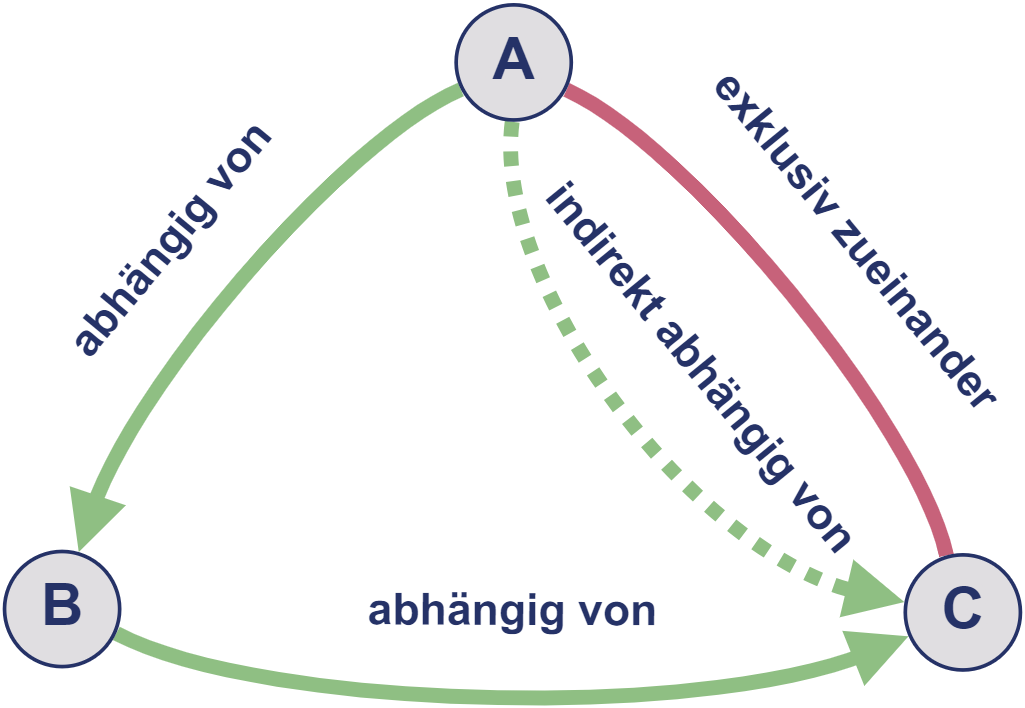
\includegraphics[width=\linewidth]{dependency_example_1.png}
      		\caption{Eine Möglichkeit, wie ein Widerspruch zwischen indirekter Abhängigkeit und Exklusivität entstehen kann.}
		\end{subfigure}
		\begin{subfigure}[a]{0.4\linewidth}
			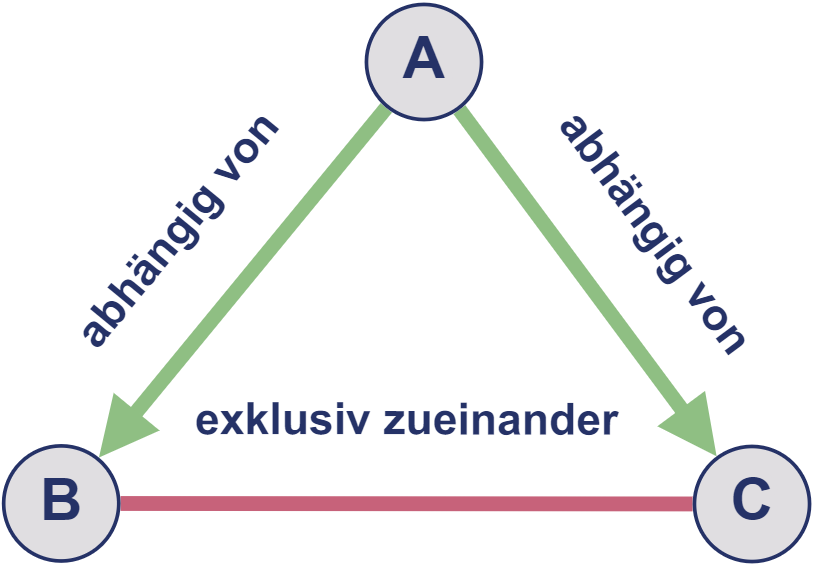
\includegraphics[width=\linewidth]{dependency_example_2.png}
      		\caption{Hier entsteht ein Widerspruch dadurch, dass eine Erweiterung zwei Abhängigkeiten hat, die zueinander exklusiv sind.}
		\end{subfigure}
		\caption{Zwei Graphen zur Veranschaulichung von Konfliktmöglichkeiten zwischen Abhängigkeiten und Exklusivitäten.}
		\label{fig:impl:dependency_conflict_examples}
  \end{figure}

Der zweite in Abbildung \ref{fig:impl:dependency_conflict_examples} dargestellte Konflikt beruht im Gegensatz zu den bisherigen Beispielen nicht darauf, dass eine Erweiterung zugleich (indirekt) abhängig von und exklusiv zu einer anderen Erweiterung ist. Hier wird eine weitere Kategorie von Problemen dargestellt: sind zwei (indirekte) Abhängigkeiten einer Erweiterung zueinander exklusiv, so können nicht beide dieser Abhängigkeiten erfüllt werden. Auch solche Konfigurationen sind also unzulässig.

Aus diesen fachlichen Überlegungen heraus ergibt sich eine erste Lösung. Für jede Erweiterung $E$ sind zunächst alle direkten sowie indirekten Abhängigkeiten zu bestimmen. Für alle diese Abhängigkeiten ist dann zu prüfen, dass zum einen die Abhängigkeit $A$ nicht zu $E$ exklusiv ist, aber auch dass $A$ zu keiner weiteren (indirekten) Abhängigkeit $A'$ von $E$ exklusiv ist.

Bei näherer Betrachtung dieser Lösung lässt sich jedoch einiges an Ineffizienz feststellen. Zum einen werden für jede Erweiterung erneut die transitiven Abhängigkeiten berechnet. Aufgrund eben dieser Transitivität sind jedoch die Berechnungen für alle Erweitungen, die Abhängigkeit einer anderen Erweiterung sind, redundant. Im schlimmsten Fall (nämlich, wenn eine Erweiterung von insgesamt $n$ Erweiterungen von allen anderen Erweiterungen (indirekt) abhängt) ist also genau eine der durchgeführten Berechnungen wirklich notwendig und $n - 1$ Berechnungen werden unnötigerweise durchgeführt. Aus ähnlichem Grund ist auch die Überprüfung der Exklusitivät zweier paarweise verschiedenen (indirekter) Abhängigkeiten häufig überflüssig.

Die Lösung dieser Probleme ergibt sich aus einer theoretischeren Betrachtung des Problems. Wie bereits aus der Verwendung des Begriffs der Transitivität hervorgeht, lassen sich Abhängigkeit und Exklusitivät als mathematische Relationen über der Menge aller Erweiterungen auffassen. Hierbei ist besonders hervorzuheben, dass die Exklusivität symmetrisch ist (ist $A$ zu $B$ exklusiv, so ist auch $B$ zu $A$ exklusiv) während Abhängigkeit nicht symmetrisch ist (im Gegenteil: bei der anfänglichen Analyse von möglichen Bibliotheken, Frameworks etc. ergab sich, dass Abhängigkeit nie symmetrisch zu sein scheint). Allerdings ist Exklusivität a priori nicht transitiv (auch, wenn $A$ zu $B$ und $B$ zu $C$ exklusiv ist, können $A$ und $C$ zusammen verwendet werden), während Abhängigkeit sehr wohl transitiv ist (wie bereits erläutert).

Vor diesem Hintergrund lässt sich erkennen, dass die Bestimmung der indirekten Abhängigkeiten der Bestimmung der transitiven Hülle gleichkommt. Diese kann mittels des Floyd-Warshall-Algorithmus (in der Warshall-Variante) berechnet werden \cite{warshal1_algorithm}. Hierfür muss zunächst ein gerichteter Graph erzeugt werden, in den alle deklarierten Abhängigkeiten als Kante eingefügt werden. Von diesem Graphen wird dann die transitive Hülle bestimmt, in der zwei Knoten $A$ und $B$ genau dann durch eine von $A$ nach $B$ gerichtete Kante verbunden sind, wenn die Erweiterung $A$ von $B$ abhängt. Der Floyd-Warshall-Algorithmus benötigt den Graphen in Form einer Adjazenzmatrix.

Auch die Relation der Exklusivität lässt sich in einen Graphen überführen. In diesem Graphen gibt es ebenfalls pro Erweiterung einen Knoten und jede Exklusivität wird als Kante dargestellt. Aufgrund der Symmetrie der Exklusivität kann dieser Graph aber ungerichtet sein.

Das Problem der Überprüfung simultaner Exklusitivät und Abhängigkeit reduziert sich nun darauf, sicherzustellen, dass es zwischen zwei Knoten (also zwischen zwei Erweiterungen) in maximal einem der beiden Graphen eine Kante gibt, wobei die Richtung keine Rolle spielt (denn wenn die Knoten exklusiv zueinander sind, darf es zwischen beiden keine Abhängigkeit geben -- egal, in welche Richtung).

Anders formuliert, darf es im Graphen der Exklusivitäten keine Kante $\{A, B\}$ geben, für die in der transitiven Hülle der Abhängigkeiten die Kante $(A, B)$ oder die Kante $(B, A)$ existiert. Da die transitive Hülle als Adjazenzmatrix vorliegt, während die Exklusivitäten als Kantenliste vorliegen, kann bei $m$ Exklusivitäten in $\mathcal{O}(m)$ über die Exklusivitäten iteriert werden und jeweils in $\mathcal{O}(1)$ die Existenz einer transitiven Abhängigkeit geprüft werden. Die Vertauschung der Reihenfolge, also die Iteration über transitive Abhängigkeiten und dann die Prüfung der Existenz einer Exklusivität, würde bei $n$ Erweiterungen einen Aufwand von $\mathcal{O}(n^2)$ verursachen. Wenn vorher die Kantenliste der Exklusivitäten in $\mathcal{O}(n^2)$ in eine Adjazenzmatrix überführt wird, ist die anschließende Existenzprüfung auch wieder in $\mathcal{O}(1)$ möglich, aber dennoch ist ersteres Vorgehen effizienter.

Der Algorithmus von Floyd-Warshall sorgt dafür, dass diese Überprüfung eine asymptotische Laufzeit von $\mathcal{O}(n^3)$ hat. Da die oben beschriebenen Probleme in beliebiger Tiefe von Abhängigkeiten auftreten können, ist jedoch die Bestimmung der transitiven Hülle nicht vermeidbar. Allerdings ist damit zu rechnen, dass die Anzahl aller Erweiterungen stets kleiner als $100$ sein wird (andernfalls würde die Benutzbarkeit des Programms möglicherweise stark eingeschränkt). Daher ist diese Laufzeit in diesem Fall als unbedenklich einzustufen.

Die Überprüfung der anderen vorgestellten Widerspruchsart, in der zwei (transitive) Abhängigkeiten einer Erweiterung zueinander exklusiv sind, lässt sich so umformulieren, dass sie ebenfalls die transitive Hülle verwendet. Darüber hinaus wurde jedoch kein Weg gefunden, ihre Laufzeit zu optimieren.

Da auch diese Überprüfung sich lediglich auf die Definitionen der Erweiterungen verlässt, wird auch sie in die Ausführung der automatisierten Tests eingebunden. So kann sichergestellt werden, dass keine fehlerhaften Erweiterungsdefinitionen veröffentlicht werden, ohne die normale Ausführungszeit zu beeinflussen.

\subsubsection{Überprüfung der getroffenen Auswahl von Erweiterungen}
\label{impl:verify_chosen_extensions}
Um die getroffene Auswahl an Erweiterungen auf die Einhaltung aller Restriktionen hin zu überprüfen, wurde ebenfalls zunächst eine fachliche Lösung gefunden. Für jede der ausgewählten Erweiterungen sind alle Abhängigkeiten und Exklusivitäten durchzugehen. Ist eine Abhängigkeit nicht mit ausgewählt worden oder ist eine Exklusivität mit ausgewählt worden, so ist (genau dann) die Kombination ungültig.

Die Laufzeit dieses Vorgehens liegt für $n$ mögliche Erweiterungen in $\mathcal{O}(n^3)$ (mit Möglichkeit der Reduktion auf $\mathcal{O}(n^2)$). Dies liegt daran, dass zunächst über jede der (maximal $n$) ausgewählten Erweiterungen und dann über jede der Abhängigkeiten und Exklusivitäten iteriert werden muss. Da eine Erweiterung niemals zu einer Abhängigkeit exklusiv sein kann, beträgt die Summe der Abhängigkeiten und Exklusivitäten maximal $n$. Somit ist bereits eine Laufzeit von $\mathcal{O}(n^2)$ erreicht worden.

Nun bleibt noch die Prüfung, ob eine Abhängigkeit bzw. Exklusivität ausgewählt worden ist oder nicht, d.h. ob sie in der Liste der ausgewählten Erweiterungen liegt oder nicht. Im Falle einer normalen Liste läge die Laufzeit dieser Überprüfung bei $\mathcal{O}(n)$, da die im schlimmsten Fall die gesamte Liste überprüft werden müsste. Allerdings kann diese Information auch als Liste bool'scher Werte gespeichert werden, wobei unter jedem Index genau eingetragen ist, ob die Erweiterung mit demselben Index in der Liste aller möglichen Erweiterungen ausgewählt worden ist. So wäre die Überprüfung der Auswahl einer einzelnen Erweiterung in $\mathcal{O}(1)$ möglich und würde die Gesamtlaufzeit nicht weiter beeinflussen.

Ähnlich wie bei der Überprüfung der Umsetzbarkeit aller Restriktionen lässt sich jedoch auch für dieses Problem eine graphentheoretische Lösung finden. Da bereits Graphen bestimmt wurden, in denen Kanten für Abhängigkeit und Exklusivität eingetragen sind, können diese zunächst kopiert und dann zur Überprüfung dieses Problems verwendet werden. Die Kopie erfolgt in $\mathcal{O}(n^2)$, da eine $n \times n$-Adjazenzatrix und eine Kantenliste mit maximal Länge $n^2$ kopiert werden müssen.

Im Graphen der Abhängigkeiten sind Kanten nun als noch unerfüllte Bedingungen anzusehen. Die Streichung einer Kante bedeutet somit, dass die entsprechende Bedingung erfüllt ist. Nun ist über jede mögliche Erweiterung zu iterieren. Falls sie ausgewählt worden ist, so sind auf sie eingehende Kanten aus dem Graphen der Abhängigkeiten zu streichen. Andernfalls (d.h. wenn sie nicht ausgewählt worden ist) ist ihr Knoten mitsamt seiner ausgehenden Kanten zu streichen. Es sind genau dann alle Abhängigkeiten erfüllt, wenn nach der Iteration über alle möglichen Erweiterungen keine Kanten mehr in dem Graphen vorhanden sind.

Ähnlich ist für die Exklusivitäten zu verfahren. In diesem Graphen bedeutet die Existenz einer Kante, dass die zugehörige Exklusivität in der aktuellen Auswahl noch nicht ausgeschlossen werden konnte. Während über alle Erweiterungen iteriert wird, kann also für jede nicht ausgewählte Erweiterung der zugehörige Knoten zusammen mit seinen (ungerichteten) Kanten gestrichen werden. Auch die Exklusivitäten sind alle genau dann erfüllt, wenn sich am Ende der Iterationen keine Kante mehr im Graphen befindet.

Der erste Aspekt der Laufzeit dieser Verfahren ergibt sich dadurch, dass die Graphen in verwendbarer und modifizierbarer Form vorliegen müssen (d.h. als neu angelegte Adjazenzmatrizen). Die im letzten Kapitel berechnete Adjazenzmatrix der Abhängigkeit muss also lediglich kopiert werden, während der Graph der Exklusivität in eine Adjazenzmatrix überführt werden muss. Dies kann in $\mathcal{O}(n^2)$ geschehen.

Danach muss über jede Erweiterung iteriert werden und ggf. (also falls sie nicht ausgewählt wurde) die zugehörige Zeile und Spalte der Adjazenzmatrix modifiziert werden. Anschließend muss die gesamte Matrix auf die Existenz von Kanten hin überprüft werden. Beide Schritte geschehen nacheinander in jeweils $\mathcal{O}(n^2)$. Somit fordert der gesamte Prozess eine Laufzeit von $\mathcal{O}(n^2)$.

Alternativ zu den Adjazenzmatrizen könnten auch Kantenlisten verwendet werden. Dann müsste aber für die Löschung von Knoten, die in beiden Prozessen maximal für jede Erweiterung vorkommen könnte, jeweils die gesamte Liste durchlaufen werden. Es entstünde also auch hier ein Aufwand von $\mathcal{O}(n^2)$.

Die Betrachtung der Graphentheoretischen Lösung ergibt also in diesem Fall keine Verbesserung der Laufzeit. Nach persönlichem Empfinden ist die erste Lösung jedoch leichter zu verstehen und wurde angesichts der gleichen Laufzeit aufgrund dieses Kriteriums ausgewählt und umgesetzt.


\subsection{Implementierung konkreter Erweiterungen}
Um die Funktionsfähigkeit des entworfenen Erweiterungssystems zu demonstrieren, werden exemplarisch einige Erweiterungen entwickelt. Zunächst werden die Installationen von React und Angular umgesetzt. Dadurch werden zwei der drei betrachteten Frameworks von \gls{GWA} unterstützt. Vue als fehlendes Framework verfügt über einen Installationsprozess, der dem von Angular sehr ähnelt, weshalb seine Implementierung keine neuen Konzepte erfordern würde.

Die initiale Projekterzeugung für beide Frameworks erfolgt über \verb/npx/, einem Hilfsbefehl von \gls{npm}, der ein gewünschtes Paket temporär herunterlädt, installiert und sofort ausführt. Diesen Befehl werden auch weitere Erweiterungen nutzen, um stets die aktuellen Versionen von Bibliotheken und Werkzeugen zu installieren.

Aufgrund seiner zentralen Stellung wird als nächstes eine Erweiterung für TypeScript implementiert. Da alle untersuchten Frameworks jedoch ggf. TypeScript mitinstallieren, muss diese Erweiterung keinen Installationsprozess durchführen. Die Erweiterung dient also zum einen als Auswahlmöglichkeit für TypeScript. Frameworks prüfen dann während ihrer Installation, ob diese Erweiterung ausgewählt wurde, um entsprechend fortzufahren.

Darüber hinaus ist TypeScript-Erweiterung jedoch in der Lage, entsprechend den Wünschen von Nutzenden die TypeScript-Kompilerkonfiguration anzupassen. Diese Konfigurationen werden in einer \gls{JSON}-Datei vorgenommen. Diese Dateien zu bearbeiten ist aufgrund der tiefen Integration von \gls{JSON} in JavaScript in der Regel sehr simpel; allerdings verfügt diese Spezielle Datei über zusätzliche Syntax zum Schreiben von Kommentaren \cite{JSON_MDN}. In den von TypeScript erzeugbaren Konfigurationsdateien sind viele solcher Kommentare vorhanden, die zudem auf eine bestimmte Weise hinter den Konfigurationszeilen eingerückt sind.

Diese Kommentare würden durch eine Bearbeitung mit den in Node.js integrierten Funktionen verloren gehen. Daher wurden eigene Funktionen geschrieben, die nur für die konkret benötigten Konfigurationseigenschaften funktionieren, aber dabei die Kommentareinrückung beibehalten können.

Als weitere Kategorie von Erweiterungen werden CSS-Präprozessoren entwickelt. Die Auswahl der unterstützten Präprozessoren ergibt sich durch die von Angular unterstützen Präprozessoren. Bis auf einen werden diese auch von React unterstützt, wobei die Installation in React-Projekten von \gls{GWA} selbst vorgenommen werden muss, während die Installation in Angular-Projekten per weitergabe eines \gls{CLI}-Argumentes geschehen kann.

Die Installation in React-Projekten erfordert drei Schritte. Zunächst müssen für die Präprozessoren benötigte \gls{npm}-Pakete installiert werden. Daraufhin werden bestimmte Dateien aus dem Projektverzeichnis durch andere, vorher festgelegte Dateien ausgetauscht werden. Die eingesetzten Dateien haben einen konstanten Inhalt, der zwischen Projekten nicht variiert. Zuletzt müssen in einigen React-Dateien die Importierungen der ausgetauschen Dateien angepasst werden.

Der Schritt der Installation von \gls{npm}-Paketen ist für viele Erweiterungen notwendig. Da der zu verwendende Paketmanager von Nutzenden ausgewählt, wird, wie in der Konzeptionierung ausgearbeitet, eine Paketmanager-Strategie entworfen, welches in Abbildung \missingQuote näher dargestellt wird. Diese wird für die beiden zu unterstützenden Paketmanager \gls{npm} und Yarn implementiert. Bei der Auswahl des Paketmanagers wird die zugehörige Strategie erzeugt und im weiteren Verlauf an sämtliche Erweiterungen gereicht, wo sie vollständig die Installation aller benötigten Pakete übernimmt.

Der Austausch der Dateien wird von Node.js-Funktionen übernommen und bedarf keiner weiteren Verallgemeinerung. Das Ändern der Importierungen wird von zwei Hilfsfunktionen übernommen, die die alten Importierungen entfernen und die neuen erzeugen, da dieser Schritt auch von anderen Erweiterungen benötigt wird.

Als Beispiel eines Werkzeuges, das ausschließlich Entwicklungszwecken dient und daher nur über Konfigurationsdateien verfügt und keine Auswirkungen auf den zu erzeugenden Produktivcode hat, wird eine Erweiterung für ESLint implementiert. Im Fall von Angular geschieht dies über ein \gls{npm}-Paket, welches erneut mit \verb/npm/ ausgeführt wird. Für sonstige Frameworks werden zunächst benötigte \gls{npm}-Pakete installiert, bevor eine an das Framework angepasste Konfigurationsdatei erzeugt wird. Diese Datei besteht größtenteils aus normalen \gls{JSON}-Daten und ist daher leicht, wie bereits erwähnt, generierbar.

Im Rahmen der letzten entwickelten Erweiterung wird Unterstützung für Redux eingebaut. Diese Erweiterung ist daher interessant, da Redux eine reine JavaScript- / TypeScript-Bibliothek ist, weshalb sich ihre Installation in einem Projekt nur auf JavaScript- / TypeScript-Code auswirkt. Um einen leichteren Einstieg in die Bibliothek zu ermöglichen, soll für alle Frameworks eine Beispielkomponente erzeugt und in die Applikation eingebunden werden, die die Verwendung der Bibliothek demonstriert.

Die Erzeugung solchen Codes stellt eine besondere Herausforderung dar, da der Code sowohl in TypeScript als auch in JavaScript erzeugbar sein muss. Auf diese Problematik wird genauer in Kapitel \ref{impl:js_from_ts} eingegangen. Darüber hinaus muss die generierte Beispielkomponente jeweils in das Projekt eingebunden werden. Da auch diese Aufgabe öfter auftreten wird, wird hierfür eine weitere Hilfsfunktion geschrieben.

\subsection{Umsetzung des Dialogs}
Der Dialog mit Nutzenden lässt sich grob in drei Aufgaben unterteilen. Die erste Aufgabe ist das Untersuchen der \gls{CLI}-Argumente. In diesem Schritt werden keine Ausgaben erzeugt, aber da er auf einer manuellen Eingabe operiert, zählt er trotzdem zum Prozess des Dialogs.

Mit den vorgegebenen Optionen werden dann, sofern notwendig, weitere allgemeine Fragen gestellt. Hier haben Nutzende die Möglichkeit, den Namen des Projektes anzugeben, einen Paketmanager und die gewünschten Erweiterungen auszuwählen. Ist eine dieser Fragen bereits in den \gls{CLI}-Argumenten beantwortet worden, so kann die entsprechende Frage übersprungen werden.

Als letzten Schritt des Dialogs sind dann weitere Fragen der einzelnen Erweiterungen zu stellen. Auch diese können bereits beantwortet worden sein und werden ggf. übersprungen.

\subsection{Analyse der CLI-Argumente}
Mithilfe der bereits erwähnten Bibliothek \glqq commander\grqq\ können die \gls{CLI}-Argumente mit sehr geringem Aufwand eingelesen und in gewissem Rahmen validiert werden. Dazu ist es notwendig, alle möglichen Argumente und ggf. die Typen der erwarteten zugehörigen Werte zu deklarieren.

Für die Angabe eines bool'schen Wertes reicht dann ein Parameter ohne zugehörigen Wert (z.B. \verb|--use-some-library|), während Angabe einer Wahl von bestimmten Optionen zusätzlich die Angabe eines Wertes benötigt (z.B. \verb|--package-manager npm|). Commander erzeugt bei der anschließenden Analyse der beim Befehlsaufruf übergebenen Argumente ein Objekt, bei dem jedem angegebenen Argument der entsprechende Wert (oder, falls kein Wert angegeben wurde, der bool'sche Wert \verb|true|) zugewiesen ist. Wenn eine Option beim Befehlsaufruf nicht angegeben wurde, so wird sie in das ausgegebene Objekt nicht aufgenommen.

Bool'sche Optionen können daher nicht durch Weglassung auf den Wert \verb|false| gesetzt werden. Um sie trotzdem negierbar zu machen, kann eine weitere Option mit dem Präfix \verb|no-| erstell werden (z.B. \verb|--no-use-some-library|). Diese wird von commander automatisch als Negation der zugehörigen Option (in dem Beispiel also der Option \verb|--use-some-library|) erkannt. Natürlich kann dieselbe Funktionalität auch mit anderen Benamungen umgesetzt werden; dies ist dann aber mit höherem Aufwand verbunden, da die zugehörige Logik von Hand implementiert werden muss.

Um alle Fragen, die im Laufe des Dialogs gestellt werden könnten, durch solche \gls{CLI}-Argumente abzudecken, muss es möglich sein, dass Erweiterungen ebenfalls Argumente deklarieren können. Dies wird umgesetzt, indem Erweiterungen eine Funktion definieren können, die auf dem überreichten commander-Objekt frei Argumente definieren kann.

Daraufhin werden die Argumente von commander analysiert. Die allgemeinen Metadaten werden herausgefiltert und an die Stellung der entsprechenden Fragen weitergegeben. Alle weiteren Argumente können im allgemeinen Teil jedoch nicht weiter verarbeitet werden und müssen daher als Gesamtheit im Rahmen des weiteren Dialogs an die Erweiterungen überreicht werden (siehe Abschnitt \ref{impl:extension_questions}).

Vor der Weitergabe der per \gls{CLI}-Argumente übergebenen allgemeinen Daten müssen diese jedoch validiert werden. Insbesondere bezieht sich dies auf die Überprüfung der Auswahl der Erweiterungen (siehe Kapitel \ref{impl:verify_chosen_extensions}). Sofern keine Erweiterung per \gls{CLI}-Argument ausgewählt wurde, kann diese Validierung übersprungen werden, da die zugehörige Frage später gestellt werden muss und die Validierung dabei erfolgen kann.

Weniger eindeutig ist jedoch, wie mit der Angabe einer oder mehrerer gewünschter Erweiterung(en) per \gls{CLI}-Argumente umzugehen ist, da nicht eindeutig erkennbar ist, ob die so getroffene Auswahl vollständig sein soll. Falls sie nicht vollständig wäre, müsste die zugehörige Frage gestellt werden, was aber eine programmatische Verwendung von \gls{GWA} deutlich erschweren würde. Daher ist davon auszugehen, dass die per \gls{CLI}-Argumente getroffene Auswahl an Erweiterungen vollständig ist, sobald mindestens eine Erweiterung ausgewählt wurde. In diesem Fall ist dann die Überprüfung dieser Auswahl durchzuführen und im Fehlerfall ist die Ausführung von \gls{GWA} abzubrechen.

\subsubsection{Stellen allgemeiner Fragen}
\label{impl:general_questions}
In diesem Abschnitt des Dialogs werden sowohl Metadaten des zu erzeugenden Projektes gesammelt als auch die Auswahl der zu installierenden Erweiterungen getroffen. Die Sammlung der Metadaten ist ohne besonderen Aufwand umsetzbar, da alle hierfür relevanten Fragetypen (Freitext-Eingabe, Auswahl eines von $n$ Elementen) von inquirer zur Verfügung gestellt werden und direkt verwendet werden können.

Bemerkenswert ist lediglich, dass vor der Frage, welcher Paketmanager verwendet werden soll, geprüft wird, welche Paketmanager überhaupt installiert sind. Auch, wenn nur ein Paketmanager installiert ist und somit gar keine Auswahl getroffen werden kann, wird die Frage gestellt und erhält lediglich ergänzende Bemerkungen, dass andere Paketmanager nicht zur Verfügung stehen. Diese Entscheidung wurde getroffen, um unerfahrene Entwickelnde zumindest darüber zu informieren, dass es weitere Paketmanager gibt. Außerdem kann diese Frage leicht übersprungen werden, indem die entsprechende Entscheidung per \gls{CLI}-Argument \verb|--package-manager| spezifiziert wird. Um dies weiter zu erleichtern, wurde auch der Alias \verb|-p| eingerichtet.

Die Frage zur Auswahl der zu installierenden Erweiterungen gestaltet sich etwas schwieriger. Sie muss von einer allgemeinen Stelle aus gestellt werden, da sie erweiterungsübergreifend ist, aber muss dennoch erweiterungsspezifische Inhalte darstellen können. Um auch diese Frage möglichst verständlich und informativ zu gestalten, müssen Erweiterungen neben ihrem Namen auch eine Kurzbeschreibung, einen Link zu mehr Informationen und die Kategorie der Erweiterung angeben. Name, Kurzbeschreibung und Link werden in die Frage eingebaut, während die Kategorie lediglich für eine sinnvolle Gruppierung und Trennung der Erweiterungen genutzt wird.

Inquirer ermöglicht bei allen Fragen die Angabe einer Funktion, die eine Antwort auf die Frage entgegennimmt und diese validiert. Auf diesem Weg ist es möglich, die in Kapitel \ref{impl:verify_chosen_extensions} beschriebene Überprüfung der getroffenen Auswahl durchzuführen. Wird ein Fehler festgestellt, so wird dieser von inquirer ausgegeben und die Frage wird beibehalten, bis eine Antwort die Validierung besteht. So wird garantiert, dass die weiteren Schritte von \gls{GWA} nicht ausgeführt werden können, bis eine gültige Auswahl von Erweiterungen getroffen wurde.

\subsubsection{Übergabe des Dialogs an Erweiterungen}
\label{impl:extension_questions}

Da auch Erweiterungen in der Lage sein müssen, im Rahmen des Dialogs Fragen zu stellen, können sie eine Funktion definieren, die nach dem Stellen eventueller Fragen ein Objekt zurück gibt, das die aus den Fragen resultierende Konfiguration enthält. Damit keine bereits beantworteten Fragen gestellt werden und die per \gls{CLI}-Argumente spezifizierten Optionen bei der Erzeugung dieses Konfigurationsobjektes berücksichtigt werden können, müssen alle \gls{CLI}-Argumente ebenfalls an diese Funktion übergeben werden.

Um den Dialog möglichst übersichtlich zu gestalten, ist es sinnvoll, die Fragen einzelner Erweiterungen visuell voneinander zu trennen, damit Nutzenden bewusst ist, worauf sich jede aktuelle Frage bezieht. Hierfür soll vor den Fragen jeder Erweiterung der Name der Erweiterung als Überschrift der folgenden Fragen ausgegeben werden. Außerdem soll zwischen den Fragen der letzten Erweiterung und der Überschrift der Fragen der nächsten Erweiterung eine Leerzeile eingefügt werden.

Um diese Formatierung zu garantieren und möglichst wiederholungsfreien Code zu erzeugen, ist diese Formatierung außerhalb der Erweiterungen umzusetzen. Dies hat zudem den Vorteil, dass Randfälle (z.B. Ausgaben vor der ersten / nach der letzten Erweiterung) leichter betrachtet werden können, da Erweiterungen beim Stellen von Fragen nicht wissen, ob vor oder Nach ihnen Fragen gestellt wurden / werden.

Diese Umsetzung ist jedoch fehlerhaft, falls aufgrund von \gls{CLI}-Argumenten bestimmte Fragen ausgesetzt werden. Wenn alle Fragen einer Erweiterung ausgesetzt werden, dann sollte für die Erweiterung auch keine Leerzeile oder Überschrift ausgegeben werden, was bei dem bisher beschriebenen Ansatz aber geschehen würde.

Um dieses Problem zu lösen, wird an die Funktionen zum Stellen von Fragen als weiterer Parameter eine Funktion übergeben, die zunächst nur inquirer ummantelt und jeden Aufruf direkt weiterleitet. Vor der Weiterleitung eines Aufrufes prüft sie jedoch, wie viele Fragen gestellt werden. Sobald eine Erweiterung (mindestens) eine Frage stellt, gibt sie vor dem Weiterleiten die trennende Leerzeile sowie die Überschrift aus. Stellt eine Erweiterung also keine Fragen, wird beides nicht ausgegeben.

Dieses Vorgehen hat auch den Vorteil, dass mit besonders geringem Aufwand im Rahmen der automatischen Tests das Stellen von Fragen gesteuert werden kann, ohne, dass die Ausgaben der Tests von Ausgaben von inquirer unterbrochen werden. Hierfür muss lediglich die übergebene Funktion darauf verzichten, inquirer aufzurufen und im Rahmen der Tests gewünschte Antworten ohne das Stellen entsprechender Fragen zurück geben.

\subsection{Installation von Erweiterungen}
Nachdem alle benötigten Informationen eingeholt und verifiziert worden sind, ist nun die Installation der Erweiterungen durchzuführen. Hierfür wird in einer bestimmten Reihenfolge (siehe Kapitel \ref{impl:determine_installation_order}) für jede der ausgewählten Erweiterungen zunächst geprüft, ob sie übersprungen werden soll. Falls dem nicht so ist, wird dann eine von ihr definierte Funktion zur Installation aufgerufen. Diese erhält als Parameter alle gesammelten Metadaten sowie die zum gewählten Paketmanager gehörige Strategie und eine Liste mit allen ausgewählten Erweiterungen mitsamt ihren speziell getroffenen Einstellungen.

Um Nutzenden den Fortschritt von \gls{GWA} mitzuteilen, wird vor dem Aufruf der Installationsfunktion ausgegeben, dass nun mit der Installation der entsprechenden Erweiterung begonnen wird. Diese Meldung wird nicht ausgegeben, wenn die Erweiterung übersprungen wird. Dies ist der Grund, warum das Überspringen der Installation einer Erweiterung gesondert überprüft werden muss, anstatt ggf. in der Installationsfunktion nichts auszuführen.

Im Anschluss an alle Installationen haben Erweiterungen die Möglichkeit durch eine von ihnen definierte Funktion weitere Informationen auszugeben. Dies kann beispielsweise genutzt werden, um erste Schritte mit einem Framework zu erläutern oder erneut auf die Dokumentation zu verweisen.

\subsubsection{Bestimmung der Installationsreihenfolge}
\label{impl:determine_installation_order}
Wie bereits in der Konzeptionierung erläutert wurde, muss es möglich sein, die Installationsreihenfolge der Erweiterungen festzulegen. Dabei ist nicht die Festlegbarkeit der gesamten Reihenfolge relevant, sondern es müssen lediglich gewisse Bedingungen eingehalten werden.

Beispielsweise muss das Framework zuerst installiert werden, da es die notwendige Ordnerstruktur erzeugt. Die Installation von husky und ESLint sollte sehr spät erfolgen, damit alle im Projekt existierenden Dateiendungen bei entsprechenden Skripten berücksichtigt werden können. Dies sind also zwei Beispiele für \glqq globale\grqq\ Bedingungen die von einer Erweiterung an den gesamten Kontext gestellt werden.

Es gibt aber auch eine weitere Art von Bedingung, bei der eine Erweiterung nicht vor einer anderen Erweiterung installiert werden darf. Ein solches Beispiel ist, dass husky nach Prettier und ESLint installiert werden muss, da sonst bei den durch husky eingerichteten Automatisierungen die anderen Werkzeuge nicht einbezogen werden. Dieses Konzept ähnelt dem der Abhängigkeiten, kann jedoch ausdrücklich nicht durch die bereits existierenden Abhängigkeiten zwischen Erweiterungen abgebildet werden. Sonst müsste beispielsweise TypeScript vor Angular installiert werden, da Angular von TypeScript abhängig ist. Dies ist jedoch nicht möglich, da (wie bereits erläutert) Frameworks als allererstes installiert werden müssen.

Obwohl sich diese Anforderungen wie geschehen kategorisieren lassen, stellen sie eher eine Ansammlung von Einzelfällen dar. Neben Frameworks gibt es keine Erweiterungen, die als erstes oder letztes zu installieren sind. Die Anforderung von Husky und ESLint ist nach bisherigem Kenntnisstand ebenfalls ein Einzelfall. Da nur begrenzt viele Bibliotheken und Werkzeuge analysiert wurden, kann es darüber hinaus sein, dass es noch weitere Arten von Bedingungen an die Installationsreihenfolge gibt, die für zukünftige Erweiterungen relevant werden. Die einzige Anforderung, die häufig festgestellt wurde, war die, dass eine Erweiterung nicht vor einer oder mehreren anderen installiert werden darf.

Alternativ kann durch händisches Festlegen der Installationsreihenfolge gewährleistet werden, dass sämtliche Anforderungen erfüllt werden. Dieser Ansatz hat den Nachteil, dass er unübersichtlicher ist und leichter bei der Ergänzung neuer Erweiterungen Fehler gemacht werden können. Dafür ist der Implementierungsaufwand deutlich geringer.

Insbesondere, da die Implementierung der bisher beobachteten Anforderungen in Form von inhaltlichen Regeln keine Zukunftssicherheit bietet und dennoch deutlich komplexer wäre, wurde nach der zweiten vorgestellten Methode vorgegangen. Alle Auswählbaren Erweiterungen wurden in einem Array derart aufgelistet, dass die Reihenfolge der Erweiterungen in dem Array die Installationsreihenfolge festlegt. Dieses Array wird zugleich überall dort verwendet, wo eine vollständige Liste aller Erweiterungen benötigt wird.

\subsubsection{Erzeugung von TypeScript- und JavaScript-Dateien}
\label{impl:js_from_ts}
Im Rahmen der Installation vieler Erweiterungen sind JavaScript- bzw. TypeScript-Dateien (mit entsprechendem Code) zu erzeugen. Hierfür lassen sich trivialerweise Beispieldateien anlegen, von denen dann gemäß der getroffenen Auswahl die richtige ausgewählt und in das neue Projekt kopiert wird. Dieser Ansatz hat jedoch den Nachteil, dass er viel Code verursachen würde, der (bis auf die Existenz von Typen) dupliziert wäre. Das würde die Wartung etwas aufwändiger und unangenehmer machen.

Zudem könnten zwei in diesem Sinne äquivalente Dateien versehentlich verschieden bearbeitet werden, sodass in nur einer der beiden Dateien ein Fehler eingeführt wird. Derartige Fehler können nur durch sehr ausgiebiges Testen gefunden werden und bleiben daher leicht unbemerkt.

Aus diesen Gründen wurde ein Ansatz entwickelt, der aus nur einer Vorlage sowohl entsprechende JavaScript- als auch TypeScript-Dateien erzeugen kann. Mithilfe des TypeScript-Kompilers, der ohnehin aus Entwicklungsgründen in das Projekt eingebunden ist, kann TypeScript-Code zu JavaScript-Code umgewandelt werden. Der Kompiler akzeptiert dabei ein Konfigurationsobjekt, in dem festgelegt werden kann, mit welcher Version des EcmaScript-Standards das JavaScript kompatibel sein soll. Indem hier der neuste Standard spezifiziert wird, ähnelt der resultierende JavaScript-Code weitestgehend bis auf die Typinformationen dem ursprünglichen Code.

Beim Kompilieren werden jedoch zuvor vorhandene Leerzeilen entfernt, die aus Formatierungs- und Verständlichkeitsgründen relevant sind. Viele dieser Zeichen lassen sich wieder einfügen, indem das Kompilat mit Prettier formatiert wird. Bei einigen Durchläufen dieses Prozesses mit verschiedenen Dateien ist jedoch aufgefallen, dass Leerzeilen, die zur gedanklichen Trennung von Codeblöcken eingefügt wurden, nicht von Prettier wiederhergestellt werden konnten.

Um auch diese Leerzeilen in die generierten JavaScript-Dateien aufnehmen zu können, wird nach dem Kompilieren das Kompilat mit dem ursprünglichen Code verglichen. Dadurch werden entfernte Leerzeichen / -zeilen gefunden und wieder in das Kompilat eingefügt. Hierbei werden jedoch in bestimmten Fällen zu viele Zeichen eingefügt (z.B. werden Leerzeilen, die aufgrund von Typdefinitionen notwendig waren, eingefügt, obwohl die Typdefinitionen nicht mehr vorhanden sind und damit die Leerzeichen / -zeilen nicht benötigt werden). Diese überflüssigen Zeichen können jedoch zuverlässig mit Prettier entfernt werden, solange der ursprüngliche Code den Formatierungsregeln entspricht, mit denen Prettier aufgerufen wird.

Auf diese Art und Weise ist es also möglich, Dateivorlagen in TypeScript zu schreiben und zu pflegen, die bei der Projektinstallation entweder direkt kopiert oder zunächst zu JavaScript umformatiert und dann in das neue Projekt eingefügt werden. Durch die Verwendung des tatsächlichen TypeScript-Kompilers kann garantiert werden, dass die auf diese Art erzeugten Dateien dieselbe Funktionalität bieten.

\subsubsection{Framework-spezifische Codegeneration}
Neben solchem Allgemeinen JavaScript- / TypeScript-Code muss für einige Erweiterungen auch Framework-spezifischer Code erzeugt werden. Dies ist vor allem dann der Fall, wenn Komponenten oder CSS-Bibliotheken zum Projekt hinzugefügt werden sollen.

Die Anforderungen, die hierfür existieren, sind zwischen den Frameworks teilweise unterschiedlich. In allen Frameworks gibt es jedoch eine Datei, in der das Einstiegselement der \gls{DOM}-Struktur erzeugt wird (in Angular ist dies die \verb|src/app/app.component.html|, in React ist es die \verb|src/App.tsx| und in Vue.js ist es die \verb|src/App.vue|), in die neue Komponenten einzufügen sind.

Dieses Einfügen neuer Komponenten soll immer an derselben Stelle erfolgen, sodass sich dort alle neuen, durch Erweiterungen hinzugefügten Komponenten nacheinander ansammeln. Eine Fachlich orientierte Lösung wäre also in der Lage, die genannten Dateien korrekt zu parsen. Änderungen würden auf dem resultierenden abstrakten Syntaxbaum vorgenommen werden, bevor aus diesem wieder der ursprüngliche Code zzgl. der Modifikationen erzeugt würde. Die so vorgenommenen Änderungn sollten minimal und korrekt formatiert sein.

Alternativ dazu wäre es, da diese entsprechenden Dateien bei jeder Installation gleich sind, möglich, über reine Textsuche die Stelle zu finden, in der die neue Komponente einzusetzen ist. Dort würde der entsprechende Code eingefügt werden und anschließend würde mithilfe von Prettier die korrekte Formatierung der Datei gewährleistet werden.

Aufgrund der verschiedenen Syntaxen der drei Frameworks müsste beschriebene fachliche Lösung für jedes Framework einzeln entwickelt werden, was nur mit hohem Aufwand umsetzbar wäre. Der Text-basierte Ansatz wäre sehr fragil, da bereits geringfügige Änderungen der durch Frameworks erzeugten Dateien dazu führen könnten, dass neue Komponenten nicht mehr eingefügt werden können.

Da aber auch der fachliche Ansatz von der genauen \gls{DOM}-Struktur abhängt, die erzeugt werden würde, ist auch er für solche Fehler anfällig. Aufgrund der deutlich geringeren Komplexität wurde deshalb der Text-basierte Ansatz bevorzugt und für alle Frameworks implementiert.

Neben dem Einfügen von Komponenten gibt es noch weitere Änderungen, die vornehmbar sein müssen. In einem Angular-Projekt muss es möglich sein, bestimmte Arrays in einer TypeScript-Datei zu modifizieren. In React-Projekten hingegen muss es möglich sein, neue \gls{DOM}-Elemente derart hinzuzufügen, dass sie andere (bereits existierende) Elemente umgeben. Beide Probleme wurden ebenfalls aus den bereits beschriebenen Gründen mit text-basierten Ansätzen gelöst.

\subsection{Probleme}
Während der Entwicklung sind einige Probleme aufgetreten, mit denen bei der Konzeptionierung nicht gerechnet worden ist. Die folgenden Unterkapitel beschreiben diese Probleme und wie sie gelöst worden sind.

\subsubsection{Falsche Typdefinitionen von inquirer}
\label{inquirer_type_issue}

Wie bereits beschrieben worden ist, wurde für die Entwicklung von \gls{GWA} TypeScript verwendet. Da aber einige der verwendeten Bibliotheken, darunter inquirer \cite{inquirer_package_json}, nicht in TypeScript entwickelt wurden und auch keine eigenen von Hand erzeugten Typdefinitionen beinhalten, müssen diese Typdefinitionen aus dritten Quellen bezogen werden.

Dieses Problem ist weit verbreitet und kann häufig mittels des DefinitelyTyped-Projektes gelöst werden. Dies ist ein großes Projekt, was für derartige \gls{npm}-Pakete Typdefinitionen sammelt und als gesonderte \gls{npm}-Pakete veröffentlicht \cite{DT_github}.

\begin{lstlisting}[caption={TypeScript-Fehlermeldung bei der Verwendung von inquirer mit einem RxJS-Observable}, captionpos=b, label={code:inquirer_ts_error}]
TS2345: Argument of type
'Observable<DistinctQuestion<Answers>>' is not assignable to
parameter of type 'QuestionCollection<Answers>'.
  Type 'Observable<DistinctQuestion<Answers>>' is missing the
  following properties from type
  'Observable<DistinctQuestion<Answers>>':
  _isScalar, _trySubscribe, _subscribe
\end{lstlisting}

Zu Beginn der Entwicklung ist der in Listing \ref{code:inquirer_ts_error} aufgeführte TypeScript-Fehler entstanden, der sich nicht durch Fehler im selbstgeschriebenen Code erklären lies. Besonders ungewöhnlich an dem Fehler ist, dass zwei identisch benannte Typen (woraus in der Regel folgt, dass die Typen auch tatsächlich identisch sind) zueinander inkompatibel sind.

Bei Nachforschungen in den Abhängigkeiten, aus denen die beiden betroffenen Werte stammten, stellte sich heraus, dass zwei Verschiedene Versionen von RxJS verwendet wurden, deren Typdefinitionen zueinander inkompatibel waren. Konkret hatten die aus DefinitelyTyped stammenden Typdefinitionen von inquirer eine Abhängigkeit auf eine veraltete Version von RxJS deklariert, während \gls{GWA} von der aktuellen Version abhängig war.

Dieser Fehler lässt sich auf zwei Wege lösen. Durch die einfache Löschung der lokalen Installation der veralteten Version von RxJS wird automatisch in den Typdefinitionen von inquirer die (weiterhin installierte) aktuelle Version von RxJS verwendet. Diese Lösung hat allerdings den Nachteil, dass die Löschung der veralteten Version nach jeder Installation oder Verlinkung von \gls{GWA} mit \gls{npm} erneut vorgenommen werden muss, da sie im Rahmen der entsprechenden Befehle erneut installiert wird.

Alternativ kann die Abhängigkeit der Typdefinitionen von inquirer aktualisiert werden. Hierfür wurde in dem DefinitelyTyped-Repository ein Pullrequest gestellt\footnote{\url{https://github.com/DefinitelyTyped/DefinitelyTyped/pull/54885}}, der aber aufgrund mehrerer anderer Abhängigkeiten auf diese Typdefinitionen besondere Überprüfung erforderte.

Während diese Überprüfung stattfand, konnte das Problem mit dem ersten Lösungsansatz umgangen werden. Seit der am 6. September 2021 veröffentlichten Version 8.1.0 der Typdefinitionen von inquirer ist das Problem jedoch gänzlich gelöst.

% TODO: vielleicht anderen begriff finden?
\subsubsection{Umgebungsbasierte Probleme}
Im Rahmen der meisten Installationsprozesse müssen verschiedene \gls{npm}-Pakete als Befehle ausgeführt werden. Beispielsweise wird zum Installieren von React der Befehl \verb/npx create-react-app <Projektname>/ ausgeführt. Hierfür wird die Node.js-interne Bibliothek \verb/child_process/ verwendet. Diese ermöglicht das Erzeugen und überwachen von neuen Prozessen.

In Unix-basierten Betriebssystemen wie Linux oder macOS lässt sich mit dieser Bibliothek problemlos der beispielhaft genannte Befehl \verb/npx create-react-app <Projektname>/ ausführen. Auf einem Windows-Computer hingegen führt der Aufruf zu einem Fehler.

Das durch diesen Befehl aufgerufene Programm \verb/npx/ kann in Unix-basierten Betriebssystemen direkt in einem neuen Prozess gestartet werden. Es liegt in Form einer JavaScript-Datei vor, an deren Beginn deklariert wird, dass diese von Node.js ausgeführt werden muss. Ist Node.js installiert, so geschieht dies automatisch.

Auf Windows-Computern wird \verb/npx/ jedoch als \verb/.cmd/-Datei installiert. Diese sind in Windows nicht direkt in einem Prozess ausführbar, sondern können nur von der Kommandozeile (der CMD) ausgeführt werden \cite{windows_spawn_cmd}. Es muss also zunächst in einem neuen Prozess die CMD aufgerufen werden, damit diese dann \verb/npx/ ausführen kann.

Aufgrund dessen, dass die Entwicklung ausschließlich in einer Unix-basierten Umgebung\footnote{Es wurde zwar ein Windows-Computer genutzt, auf dem aber Windows Subsystem for Linux (\url{https://docs.microsoft.com/en-us/windows/wsl/about}) installiert war. Die Entwicklung hat ausschließlich in einer damit eingerichteten Virtuellen Maschine mit Ubuntu stattgefunden.} stattfand, ist dieser Fehler nur aufgefallen, als Dritte \gls{GWA} auf eigenen Computern getestet haben. Daraufhin wurde darauf geachtet, \gls{GWA} sowohl in Unix-basierten Umgebungen als auch auf einem Windows-System ausgiebig zu testen, wobei weitere leicht zu lösende Probleme (wie die Verwendung falscher Trennzeichen für Ordnerstrukturen) aufgefallen sind.

Durch die Verwendung anderer Werkzeuge (wie der Framework-spezifischen \gls{CLI}s) zur Installation bestimmter Bibliotheken kann es geschehen, dass auf einem Computer vorinstallierte Versionen dieser Werkzeuge einen Einfluss auf die Ausführung von \gls{GWA} haben. Solche Einflüsse müssen ausgeschlossen werden, um ein einheitliches Verhalten des Programms gewährleisten zu können.

Außerdem muss natürlich sichergestellt werden, dass diese Abhängigkeiten auch dann verwendbar sind, wenn Nutzende sie nicht zuvor installiert haben. Da viele dieser Werkzeuge im Rahmen der Konzeptionierung installiert werden mussten, fällt es im Rahmen der Entwicklung nicht auf, wenn diese Installation nicht stattfindet sondern die Abhängigkeit fälschlicherweise als bereits installiert vorausgesetzt wird.

Um derartige Probleme auch während der Entwicklung feststellen zu können, lässt sich eine \gls{VM} erzeugen, auf der \gls{GWA} ausgeführt wird. Zum Erzeugen solcher \gls{VM}s wird Docker verwendet, da so mit einer Konfigurationsdatei festgelegt werden kann, welche Abhängigkeiten vor der Ausführung von \gls{GWA} bereits installiert sein sollen und welche nicht. Dieser Ansatz wird im Rahmen der Evaluierung (Kapitel \ref{eval}) ausführlicher erläutert, aber bereits während der Entwicklung konnten auf diese Weise fehlende Abhängigkeitsinstallationen entdeckt werden.


\end{document}
